% Options for packages loaded elsewhere
\PassOptionsToPackage{unicode}{hyperref}
\PassOptionsToPackage{hyphens}{url}
%
\documentclass[
]{book}
\usepackage{lmodern}
\usepackage{amsmath}
\usepackage{ifxetex,ifluatex}
\ifnum 0\ifxetex 1\fi\ifluatex 1\fi=0 % if pdftex
  \usepackage[T1]{fontenc}
  \usepackage[utf8]{inputenc}
  \usepackage{textcomp} % provide euro and other symbols
  \usepackage{amssymb}
\else % if luatex or xetex
  \usepackage{unicode-math}
  \defaultfontfeatures{Scale=MatchLowercase}
  \defaultfontfeatures[\rmfamily]{Ligatures=TeX,Scale=1}
\fi
% Use upquote if available, for straight quotes in verbatim environments
\IfFileExists{upquote.sty}{\usepackage{upquote}}{}
\IfFileExists{microtype.sty}{% use microtype if available
  \usepackage[]{microtype}
  \UseMicrotypeSet[protrusion]{basicmath} % disable protrusion for tt fonts
}{}
\makeatletter
\@ifundefined{KOMAClassName}{% if non-KOMA class
  \IfFileExists{parskip.sty}{%
    \usepackage{parskip}
  }{% else
    \setlength{\parindent}{0pt}
    \setlength{\parskip}{6pt plus 2pt minus 1pt}}
}{% if KOMA class
  \KOMAoptions{parskip=half}}
\makeatother
\usepackage{xcolor}
\IfFileExists{xurl.sty}{\usepackage{xurl}}{} % add URL line breaks if available
\IfFileExists{bookmark.sty}{\usepackage{bookmark}}{\usepackage{hyperref}}
\hypersetup{
  pdftitle={Szövegbányászat és mesterséges intelligencia R-ben},
  pdfauthor={Sebők Miklós, Ring Orsolya},
  hidelinks,
  pdfcreator={LaTeX via pandoc}}
\urlstyle{same} % disable monospaced font for URLs
\usepackage{color}
\usepackage{fancyvrb}
\newcommand{\VerbBar}{|}
\newcommand{\VERB}{\Verb[commandchars=\\\{\}]}
\DefineVerbatimEnvironment{Highlighting}{Verbatim}{commandchars=\\\{\}}
% Add ',fontsize=\small' for more characters per line
\usepackage{framed}
\definecolor{shadecolor}{RGB}{248,248,248}
\newenvironment{Shaded}{\begin{snugshade}}{\end{snugshade}}
\newcommand{\AlertTok}[1]{\textcolor[rgb]{0.94,0.16,0.16}{#1}}
\newcommand{\AnnotationTok}[1]{\textcolor[rgb]{0.56,0.35,0.01}{\textbf{\textit{#1}}}}
\newcommand{\AttributeTok}[1]{\textcolor[rgb]{0.77,0.63,0.00}{#1}}
\newcommand{\BaseNTok}[1]{\textcolor[rgb]{0.00,0.00,0.81}{#1}}
\newcommand{\BuiltInTok}[1]{#1}
\newcommand{\CharTok}[1]{\textcolor[rgb]{0.31,0.60,0.02}{#1}}
\newcommand{\CommentTok}[1]{\textcolor[rgb]{0.56,0.35,0.01}{\textit{#1}}}
\newcommand{\CommentVarTok}[1]{\textcolor[rgb]{0.56,0.35,0.01}{\textbf{\textit{#1}}}}
\newcommand{\ConstantTok}[1]{\textcolor[rgb]{0.00,0.00,0.00}{#1}}
\newcommand{\ControlFlowTok}[1]{\textcolor[rgb]{0.13,0.29,0.53}{\textbf{#1}}}
\newcommand{\DataTypeTok}[1]{\textcolor[rgb]{0.13,0.29,0.53}{#1}}
\newcommand{\DecValTok}[1]{\textcolor[rgb]{0.00,0.00,0.81}{#1}}
\newcommand{\DocumentationTok}[1]{\textcolor[rgb]{0.56,0.35,0.01}{\textbf{\textit{#1}}}}
\newcommand{\ErrorTok}[1]{\textcolor[rgb]{0.64,0.00,0.00}{\textbf{#1}}}
\newcommand{\ExtensionTok}[1]{#1}
\newcommand{\FloatTok}[1]{\textcolor[rgb]{0.00,0.00,0.81}{#1}}
\newcommand{\FunctionTok}[1]{\textcolor[rgb]{0.00,0.00,0.00}{#1}}
\newcommand{\ImportTok}[1]{#1}
\newcommand{\InformationTok}[1]{\textcolor[rgb]{0.56,0.35,0.01}{\textbf{\textit{#1}}}}
\newcommand{\KeywordTok}[1]{\textcolor[rgb]{0.13,0.29,0.53}{\textbf{#1}}}
\newcommand{\NormalTok}[1]{#1}
\newcommand{\OperatorTok}[1]{\textcolor[rgb]{0.81,0.36,0.00}{\textbf{#1}}}
\newcommand{\OtherTok}[1]{\textcolor[rgb]{0.56,0.35,0.01}{#1}}
\newcommand{\PreprocessorTok}[1]{\textcolor[rgb]{0.56,0.35,0.01}{\textit{#1}}}
\newcommand{\RegionMarkerTok}[1]{#1}
\newcommand{\SpecialCharTok}[1]{\textcolor[rgb]{0.00,0.00,0.00}{#1}}
\newcommand{\SpecialStringTok}[1]{\textcolor[rgb]{0.31,0.60,0.02}{#1}}
\newcommand{\StringTok}[1]{\textcolor[rgb]{0.31,0.60,0.02}{#1}}
\newcommand{\VariableTok}[1]{\textcolor[rgb]{0.00,0.00,0.00}{#1}}
\newcommand{\VerbatimStringTok}[1]{\textcolor[rgb]{0.31,0.60,0.02}{#1}}
\newcommand{\WarningTok}[1]{\textcolor[rgb]{0.56,0.35,0.01}{\textbf{\textit{#1}}}}
\usepackage{graphicx}
\makeatletter
\def\maxwidth{\ifdim\Gin@nat@width>\linewidth\linewidth\else\Gin@nat@width\fi}
\def\maxheight{\ifdim\Gin@nat@height>\textheight\textheight\else\Gin@nat@height\fi}
\makeatother
% Scale images if necessary, so that they will not overflow the page
% margins by default, and it is still possible to overwrite the defaults
% using explicit options in \includegraphics[width, height, ...]{}
\setkeys{Gin}{width=\maxwidth,height=\maxheight,keepaspectratio}
% Set default figure placement to htbp
\makeatletter
\def\fps@figure{htbp}
\makeatother
\setlength{\emergencystretch}{3em} % prevent overfull lines
\providecommand{\tightlist}{%
  \setlength{\itemsep}{0pt}\setlength{\parskip}{0pt}}
\setcounter{secnumdepth}{-\maxdimen} % remove section numbering
\ifluatex
  \usepackage{selnolig}  % disable illegal ligatures
\fi

\title{Szövegbányászat és mesterséges intelligencia R-ben}
\author{Sebők Miklós, Ring Orsolya}
\date{}

\begin{document}
\frontmatter
\maketitle

\mainmatter
\hypertarget{bevezetuxe9s}{%
\chapter{Bevezetés}\label{bevezetuxe9s}}

Jelen kötet a Kvantitatív szövegelemzés és szövegbányászat a
politikatudományban (L'Harmattan, 2016) című könyv folytatásaként és
egyben kiegészítéseként a szövegbányászat és a mesterséges intelligencia
társadalomtudományi alkalmazásának gyakorlatába nyújt bevezetést. A
szövegek kvantitatív elemzése (quantitative text analysis -- QTA) a
nemzetközi társadalomtudomány egyik leggyorsabban fejlődő irányzata. A
szövegek és más minőségi adatok (filmek, képek) elemzése annyiban
különbözik a mennyiségi (kvantitatív) adatokétól, hogy nyers formájukban
még nem alkalmasak arra, hogy statisztikai, illetve ökonometriai elemzés
alá vessük őket, s így további módszertani problémákat vetnek fel,
melyek speciális tárgyalása szükséges. A tervezett kötetben bemutatott
példák többsége a politikatudományhoz kapcsolódik, de más alkalmazási
területekre is kitér.

Míg az előző kötet az egyes kódolási eljárásokat, illetve ezek
kutatás-módszertani előnyeit és hátrányait ismertette, itt a
társadalomtudományi elemzésének során használható kvantitatív
szövegelemzés legfontosabb gyakorlati feladatait vesszük sorra. A
kézirat a magyar tankönyvpiacon az elsőnek számít a tekintetben, hogy a
társadalomtudományban használatos kvantitatív szövegelemzési eljárásokat
részletesen, lépésről-lépésre ismerteti, kezdve a megfelelő korpusz
kialakításához szükséges ismeretektől, a különböző szövegbányászati
módszerek (szózsák, dokumentum-kifejezés mátrix, a névelem-felismerés,
az osztályozás, illetve a csoportosítás feladataira), illetve az
egyszerűbb szövegösszehasonlítási-feladatok áttekintésén át, egészen a
felügyelt és felügyelet nélküli gépi tanulásig, a politikatudományi
vizsgálatok során leggyakrabban használatos R programnyelven készült
programok segítségével.

Az olvasó a két kötet együttes használatával olyan ismeretek birtokába
kerül, melyek révén képes lesz alkalmazni a kvantitatív szövegelemzés és
szövegbányászat legalapvetőbb eljárásait saját kutatására. Deduktív vagy
induktív felfedező logikája fényében dönthet az adatelemzés módjáról, és
a felkínált menüből kiválaszthatja a kutatási tervéhez legjobban
illeszkedő megoldásokat. A kötetet végigkísérő konkrét példák
segítségével pedig akár reprodukálhatja is ezen eljárásokat saját
kutatásában. Mindezt a kötet függelékében helyet kapó R-scriptek
részletes leírása is segíti majd. A kötet két fő célcsoportjaként így a
társadalomtudományi kutatói és felsőoktatási közösséget határozzuk meg,
valamint rögzítjük, hogy a kvantitatív szövegelemzés területén belül
elsődlegesen a dokumentum- és tartalomelemzési módszertanhoz
kapcsolódunk.

A könyvben ugyancsak helyet kap a fontosabb fogalmak magyar és angol
nyelvű szószedete, valamint a további olvasásra ajánlott szakirodalom
szerepeltetése. Az oktatásban való közvetlen alkalmazást segíthetik
továbbá a fejezetek végén megadott vizsgakérdések, illetve a kötet
honlapján (qta.tk.mta.hu) szereplő további információk:
gyakorlófeladatok (megoldásokkal), az egyes feladatokra alkalmazható
scriptek és kereskedelmi programok bemutatása, a témával kapcsolatos
prezentációk és további ajánlott irodalmak.

\hypertarget{a-kvantitatuxedv-szuxf6vegelemzuxe9s-uxe9s-szuxf6vegbuxe1nyuxe1szat-alapfogalmai}{%
\chapter{A kvantitatív szövegelemzés és szövegbányászat
alapfogalmai}\label{a-kvantitatuxedv-szuxf6vegelemzuxe9s-uxe9s-szuxf6vegbuxe1nyuxe1szat-alapfogalmai}}

elso fejezet

\hypertarget{az-adatkezeluxe9s-r-ben}{%
\chapter{Az adatkezelés R-ben}\label{az-adatkezeluxe9s-r-ben}}

\hypertarget{adatok-importuxe1luxe1sa-uxe9s-exportuxe1luxe1sa}{%
\section{Adatok importálása és
exportálása}\label{adatok-importuxe1luxe1sa-uxe9s-exportuxe1luxe1sa}}

Az adatok importálására az R alapfüggvénye mellett több package is
megoldást kínál. Ezek közül a könyv írásakor a legnépszerűbbek a
\texttt{readr} és a \texttt{rio} csomagok. Az egyszerűség kedvéért mi az
alap \texttt{read.csv()} függvényt fogjuk használni. Amennyiben
kihasználjuk az RStudio projekt opcióját (lásd a
\protect\hyperlink{projektmunka}{Függelékben}) akkor elegendő csak az
elérni kívánt adatok relativ elérési útját megadni (relative path).
Ideális esetben az adataink egy csv fileban vannak (comma separated
values), ahol az egyes értékeket vesszők (vagy egyéb speciális karakter)
választják el. Ez esetben a \texttt{read.csv} függvényt használjuk. A
beolvasásnál egyből el is tároljuk az adatokat egy objektumban. A
\texttt{sep\ =} opcióval tudjuk a szeparátor karaktert beállítani, mert
előfordulhat hogy vessző helyett pontosvessző tagolja az adatainkat.

\begin{Shaded}
\begin{Highlighting}[]
\NormalTok{df }\OtherTok{\textless{}{-}} \FunctionTok{read.csv}\NormalTok{(}\StringTok{"data/adatfile.csv"}\NormalTok{, }\AttributeTok{sep =} \StringTok{","}\NormalTok{)}
\end{Highlighting}
\end{Shaded}

Az R képes linkről letölteni fileokat, elég megadnunk egy működő elérési
útvonalat.

\textbf{placeholder link, cserelni majd mukodore}

\begin{Shaded}
\begin{Highlighting}[]
\NormalTok{df\_online }\OtherTok{\textless{}{-}} \FunctionTok{read.csv}\NormalTok{(}\StringTok{"https://www.qta.tk.mta.hu/adatok/adatfile.csv"}\NormalTok{)}
\end{Highlighting}
\end{Shaded}

Az R package ökoszisztémája kellően változatos ahhoz, hogy gyakorlatilag
bármilyen inputtal meg tudjon bírkózni. Az Excel fileokat a
\texttt{readxl} csomagot használva tudjuk betölteni (a csomagok
installálásával kapcsolatban lásd a
\protect\hyperlink{packages}{Függeléket}), a \texttt{read\_excel()}-t
használva. A leggyakoribb statisztikai programok formátumait pedig a
\texttt{haven} csomag tudja kezelni (például Stata, Spss, SAS). A
szintaxis itt is hasonló: \texttt{read\_stata}, \texttt{read\_spss},
\texttt{read\_sas}.

\hypertarget{szuxf6veges-dokumentumok-importuxe1luxe1sa}{%
\subsection{Szöveges dokumentumok
importálása}\label{szuxf6veges-dokumentumok-importuxe1luxe1sa}}

A nagy mennyiségű szöveges dokumentum (a legyakrabban előforduló
kiterjesztések: \texttt{.txt}, \texttt{.doc}, \texttt{.pdf},
\texttt{.json}, \texttt{.csv}, \texttt{.xml}, \texttt{.rtf},
\texttt{.odt}) betöltésére a legalkalmasabb a \texttt{readtext} package.
Az alábbi példa azt mutatja be, hogy hogyan tudunk beolvasni egy adott
mappából az összes .txt kiterjesztésű file-t, anélkül hogy bármilyen
loop-ot kellene írnunk, vagy egyenként megadni a file-ok neveit. A
\texttt{*} karakter az azt jelenti ebben a környezetben, hogy bármilyen
fájl, ami .txt-re végződik. Amennyiben a fájlok nevei tartalmaznak
valamilyen meta adatot tartalmaznak, akkor ezt be tudjuk allítani a
betöltés során. Ilyen meta adat lehet például egy parlamenti
felszólalásnál a felszólaló neve és a beszéd ideje és párttagsága
(például: \texttt{kovacsjanos\_1994\_fkgp.txt}).

\begin{Shaded}
\begin{Highlighting}[]
\NormalTok{df\_text }\OtherTok{\textless{}{-}} \FunctionTok{readtext}\NormalTok{(}
  \StringTok{"data/*.txt"}\NormalTok{, }
  \AttributeTok{docvarsfrom =} \StringTok{"filenames"}\NormalTok{, }
  \AttributeTok{dvsep =} \StringTok{"\_"}\NormalTok{,}
  \AttributeTok{docvarnames =} \FunctionTok{c}\NormalTok{(}\StringTok{"nev"}\NormalTok{, }\StringTok{"ev"}\NormalTok{, }\StringTok{"part"}\NormalTok{)}
\NormalTok{  )}
\end{Highlighting}
\end{Shaded}

\hypertarget{adatok-exportuxe1luxe1sa}{%
\section{Adatok exportálása}\label{adatok-exportuxe1luxe1sa}}

Az adatainkat R-ből a \texttt{write.csv()}-vel exportálhatjuk a kívánt
helyre, \texttt{.csv} formátumban. Az R rendelkezik saját, .Rds és .Rda
kiterjesztésű, tömörített fájlformátummal. Mivel ezeket csak az R-ben
nyithatjuk meg, érdemes a köztes, hosszadalmas számítást igénylő lépések
elmentésére használni, a \texttt{saveRDS()} és a \texttt{save()}
parancsokkal. Az \texttt{openxlsx} csomaggal \texttt{.xls} és
\texttt{.xlsx} Excel formátumokba is tudunk exportálni, hogyha
szükséges.

\hypertarget{a-pipe-operuxe1tor}{%
\section{A pipe operátor}\label{a-pipe-operuxe1tor}}

Az úgynevezett \emph{pipe} operátor alapjaiban határozta meg a modern R
fejlődését és a népszerű package ökoszisztéma, a \emph{tidyverse}, egyik
alapköve. Úgy gondoljuk, hogy a \emph{tidyverse} és a \emph{pipe}
egyszerűbbé teszi elsajátítani az R használatát, ezért mi is erre
helyezzük a hangsúlyt.\footnote{A \emph{tidyverse} megközelítés miatt a
  kötetben szereplő R kód követi a ``The tidyverse style guide''
  dokumentációt (\url{https://style.tidyverse.org/})} Vizuálisan a pipe
operátor így néz ki: \texttt{\%\textgreater{}\%} és arra szolgál hogy a
kódban több egymáshoz kapcsolódó műveletet egybefűzzűnk.\footnote{Az
  RStudio-ban a pipe operátor billentyű kombinációja a
  \texttt{Ctrl\ +\ Shift\ +\ M}} Technikailag a pipe a bal oldali elemet
adja meg a jobb oldali függvény első argumentumának. A lenti példa
ugyanazt a folyamatot írja le, az alap R (\emph{base R}) illetve a pipe
használatával.\footnote{Köszönjük Andrew Heissnek a kitűnő példát.}
Miközben a kódot olvassuk érdemes a pipe-ot ``\emph{és aztán}''-nak
fordítani.

\begin{Shaded}
\begin{Highlighting}[]
\FunctionTok{reggeli}\NormalTok{(}\FunctionTok{oltozkodes}\NormalTok{(}\FunctionTok{felkeles}\NormalTok{(}\FunctionTok{ebredes}\NormalTok{(en, }\AttributeTok{idopont =} \StringTok{"8:00"}\NormalTok{), }\AttributeTok{oldal =} \StringTok{"jobb"}\NormalTok{), }\AttributeTok{nadrag =} \ConstantTok{TRUE}\NormalTok{, }\AttributeTok{ing =} \ConstantTok{TRUE}\NormalTok{))}

\NormalTok{en }\SpecialCharTok{\%\textgreater{}\%} 
  \FunctionTok{ebredes}\NormalTok{(}\AttributeTok{idopont =} \StringTok{"8:00"}\NormalTok{) }\SpecialCharTok{\%\textgreater{}\%} 
  \FunctionTok{felkeles}\NormalTok{(}\AttributeTok{oldal =} \StringTok{"jobb"}\NormalTok{) }\SpecialCharTok{\%\textgreater{}\%} 
  \FunctionTok{oltozkodes}\NormalTok{(}\AttributeTok{nadrag =} \ConstantTok{TRUE}\NormalTok{, }\AttributeTok{ing =} \ConstantTok{TRUE}\NormalTok{) }\SpecialCharTok{\%\textgreater{}\%} 
  \FunctionTok{reggeli}\NormalTok{()}
\end{Highlighting}
\end{Shaded}

A fenti példa is jól mutatja, hogy a pipe a bal oldali elemet fogja a
jobb oldali függvény első elemének berakni. A fejezet további részeiben
még bőven fogunk gyakorlati példát találni a használatára. A fejezetben
bemutatott példák az alkalmazásoknak csak egy relatíve szűk körét
mutatják be, ezért érdemes átolvasni a csomagokhoz tartozó
dokumentációt, illetve ha van, akkor a működést demonstráló bemutató
oldalakat is.

\hypertarget{muveletek-a-date-framekkel}{%
\section{Muveletek a date framekkel}\label{muveletek-a-date-framekkel}}

A data frame az egyik leghasznosabb és leggyakrabban használt adat
tárolási mód az R-ben (a részletesebb leírás a
\protect\hyperlink{data-frame}{Függelékben} található) és ebben az
alfejezetben azt mutatjuk be a \texttt{dplyr} és \texttt{gapminder}
csomagok segíségével, hogy hogyan lehet hatékonyan dolgozni velük. A
\texttt{dplyr} az egyik legnépszerűbb R csomag, a \emph{tidyverse}
része. A \texttt{gapminder} csomag pedig a példa adatbázisunkat
tartalmazza, amiben a világ országainak különböző gazdasági és
társadalmi mutatói vannak.

\begin{Shaded}
\begin{Highlighting}[]
\FunctionTok{library}\NormalTok{(dplyr)}
\FunctionTok{library}\NormalTok{(gapminder)}
\end{Highlighting}
\end{Shaded}

\hypertarget{megfigyeluxe9sek-szux171ruxe9se-filter}{%
\subsection{\texorpdfstring{Megfigyelések szűrése:
\texttt{filter()}}{Megfigyelések szűrése: filter()}}\label{megfigyeluxe9sek-szux171ruxe9se-filter}}

A sorok (megfigyelések) szűréséhez a \texttt{dplyr} csomag
\texttt{filter()} parancsát használva lehetőségünk van arra hogy egy
vagy több kritérium alapján szűkítsük az adatbázisunkat. A lenti
példában azokat megfigyeléseket tartjuk meg, ahol az év 1962 és a
várható élettartam nagyobb mint 72 év.

\begin{Shaded}
\begin{Highlighting}[]
\NormalTok{gapminder }\SpecialCharTok{\%\textgreater{}\%}
  \FunctionTok{filter}\NormalTok{(year }\SpecialCharTok{==} \DecValTok{1962}\NormalTok{, lifeExp }\SpecialCharTok{\textgreater{}} \DecValTok{72}\NormalTok{)}
\end{Highlighting}
\end{Shaded}

\begin{verbatim}
## # A tibble: 5 x 6
##   country     continent  year lifeExp      pop gdpPercap
##   <fct>       <fct>     <int>   <dbl>    <int>     <dbl>
## 1 Denmark     Europe     1962    72.4  4646899    13583.
## 2 Iceland     Europe     1962    73.7   182053    10350.
## 3 Netherlands Europe     1962    73.2 11805689    12791.
## 4 Norway      Europe     1962    73.5  3638919    13450.
## 5 Sweden      Europe     1962    73.4  7561588    12329.
\end{verbatim}

De ugyanígy leválogathatjuk a data frame-ből az adatokat akkor is hogyha
egy karakter változó alapján szeretnénk szűrni.

\begin{Shaded}
\begin{Highlighting}[]
\NormalTok{gapminder }\SpecialCharTok{\%\textgreater{}\%}
  \FunctionTok{filter}\NormalTok{(country }\SpecialCharTok{==} \StringTok{"Sweden"}\NormalTok{, year }\SpecialCharTok{\textgreater{}} \DecValTok{1990}\NormalTok{)}
\end{Highlighting}
\end{Shaded}

\begin{verbatim}
## # A tibble: 4 x 6
##   country continent  year lifeExp     pop gdpPercap
##   <fct>   <fct>     <int>   <dbl>   <int>     <dbl>
## 1 Sweden  Europe     1992    78.2 8718867    23880.
## 2 Sweden  Europe     1997    79.4 8897619    25267.
## 3 Sweden  Europe     2002    80.0 8954175    29342.
## 4 Sweden  Europe     2007    80.9 9031088    33860.
\end{verbatim}

Itt tehát a data frame azon sorait szeretnénk látni, ahol az ország
megegyezik a „Sweden" karakterlánccal az év pedig nagyobb, mint 1990.

\hypertarget{vuxe1ltozuxf3k-kivuxe1logatuxe1sa-select}{%
\subsection{\texorpdfstring{Változók kiválogatása:
\texttt{select()}}{Változók kiválogatása: select()}}\label{vuxe1ltozuxf3k-kivuxe1logatuxe1sa-select}}

A \texttt{select()} függvény segítségével válogathatunk oszlopokat a
data frame-ből. A változók kiválasztására több megoldás is van. A
\texttt{dplyr} csomag tartalmaz apróbb kisegítő függvényeket, amik
megkönnyítik a nagy adatbázisok esetén a változók kiválogatását a nevük
alapján. Ezek a függvények a \texttt{contains()},
\texttt{starts\_with()}, \texttt{ends\_with()}, \texttt{matches()} és
beszédesen arra szolgálnak hogy bizonyos nevű változókat ne kelljen
egyenként felsorolni. A \texttt{select()}-en belüli változó sorrend
egyben az eredmény data frame változó sorrendjet is megadja. A negatív
kiválasztás is lehetséges, ebben az esetben egy \texttt{-} kell tennünk
a nemkívánt változó(k) elé (pl.:
\texttt{select(df,\ year,\ country,\ -continent}).

\begin{Shaded}
\begin{Highlighting}[]
\NormalTok{gapminder }\SpecialCharTok{\%\textgreater{}\%} 
  \FunctionTok{select}\NormalTok{(}\FunctionTok{contains}\NormalTok{(}\StringTok{"ea"}\NormalTok{), }\FunctionTok{starts\_with}\NormalTok{(}\StringTok{"co"}\NormalTok{), pop)}
\end{Highlighting}
\end{Shaded}

\begin{verbatim}
## # A tibble: 1,704 x 4
##     year country     continent      pop
##    <int> <fct>       <fct>        <int>
##  1  1952 Afghanistan Asia       8425333
##  2  1957 Afghanistan Asia       9240934
##  3  1962 Afghanistan Asia      10267083
##  4  1967 Afghanistan Asia      11537966
##  5  1972 Afghanistan Asia      13079460
##  6  1977 Afghanistan Asia      14880372
##  7  1982 Afghanistan Asia      12881816
##  8  1987 Afghanistan Asia      13867957
##  9  1992 Afghanistan Asia      16317921
## 10  1997 Afghanistan Asia      22227415
## # ... with 1,694 more rows
\end{verbatim}

\hypertarget{uxfaj-vuxe1ltozuxf3k-luxe9trehozuxe1sa-mutate}{%
\subsection{\texorpdfstring{Új változók létrehozása:
\texttt{mutate()}}{Új változók létrehozása: mutate()}}\label{uxfaj-vuxe1ltozuxf3k-luxe9trehozuxe1sa-mutate}}

Az elemzési munkafolyamat elkerülhetetlen része hogy új változókat
hozzunk létre, vagy a meglévőket módosítsuk. Ezt a \texttt{mutate()}-el
tehetjuk meg, ahol a szintaxis a következő:
\texttt{mutate(data\ frame,\ uj\ valtozo\ =\ ertekek)}. Példaként
kiszámoljuk a Svéd GDP-t (milliárd dollárban) 1992-től kezdve. A
\texttt{mutate()} alkalmazásával részletesebben is foglalkozunk a
szövegek előkészítésével foglalkozó fejezetben.

\begin{Shaded}
\begin{Highlighting}[]
\NormalTok{gapminder }\SpecialCharTok{\%\textgreater{}\%} 
  \FunctionTok{filter}\NormalTok{(country }\SpecialCharTok{==} \StringTok{"Sweden"}\NormalTok{, year }\SpecialCharTok{\textgreater{}=} \DecValTok{1992}\NormalTok{) }\SpecialCharTok{\%\textgreater{}\%} 
  \FunctionTok{mutate}\NormalTok{(}\AttributeTok{gdp =}\NormalTok{ (gdpPercap }\SpecialCharTok{*}\NormalTok{ pop) }\SpecialCharTok{/} \DecValTok{10}\SpecialCharTok{\^{}}\DecValTok{9}\NormalTok{)}
\end{Highlighting}
\end{Shaded}

\begin{verbatim}
## # A tibble: 4 x 7
##   country continent  year lifeExp     pop gdpPercap   gdp
##   <fct>   <fct>     <int>   <dbl>   <int>     <dbl> <dbl>
## 1 Sweden  Europe     1992    78.2 8718867    23880.  208.
## 2 Sweden  Europe     1997    79.4 8897619    25267.  225.
## 3 Sweden  Europe     2002    80.0 8954175    29342.  263.
## 4 Sweden  Europe     2007    80.9 9031088    33860.  306.
\end{verbatim}

\hypertarget{csoportonkuxe9nti-statisztikuxe1k-group_by-uxe9s-summarize}{%
\subsection{\texorpdfstring{Csoportonkénti statisztikák:
\texttt{group\_by()} és
\texttt{summarize()}}{Csoportonkénti statisztikák: group\_by() és summarize()}}\label{csoportonkuxe9nti-statisztikuxe1k-group_by-uxe9s-summarize}}

Az adataink részletesebb és alaposabb megismerésében segítenek a
különböző szintű leíró statisztikai adatok. A szintek megadására a
\texttt{group\_by()} használható, a csoportokon belüli számításokhoz
pedig a \texttt{summarize()}. A lenti példa azt illusztrálja, hogyha
kontinensenként csoportosítjuk a \texttt{gapminder} data framet, akkor a
\texttt{summarise()} használatával megkaphatjuk a megfigyelések számát,
illetve az átlagos per capita GDP-t. A \texttt{summarise()} a
\texttt{mutate()} közeli rokona, hasonló szintaxissal és logikával
használható. Ezt a függvény párost fogjuk majd használni a szöveges
adataink leíró statisztikáinál is a 4. fejezetben.

\begin{Shaded}
\begin{Highlighting}[]
\NormalTok{gapminder }\SpecialCharTok{\%\textgreater{}\%} 
  \FunctionTok{group\_by}\NormalTok{(continent) }\SpecialCharTok{\%\textgreater{}\%} 
  \FunctionTok{summarise}\NormalTok{(}\AttributeTok{megfigyelesek =} \FunctionTok{n}\NormalTok{(), }\AttributeTok{atlag\_gdp =} \FunctionTok{mean}\NormalTok{(gdpPercap))}
\end{Highlighting}
\end{Shaded}

\begin{verbatim}
## `summarise()` ungrouping output (override with `.groups` argument)
\end{verbatim}

\begin{verbatim}
## # A tibble: 5 x 3
##   continent megfigyelesek atlag_gdp
##   <fct>             <int>     <dbl>
## 1 Africa              624     2194.
## 2 Americas            300     7136.
## 3 Asia                396     7902.
## 4 Europe              360    14469.
## 5 Oceania              24    18622.
\end{verbatim}

\hypertarget{munka-karakter-vektorokkaladatkezeles-4}{%
\section[Munka karakter vektorokkal]{\texorpdfstring{Munka karakter
vektorokkal\footnote{A könyv terjedelme miatt ezt a témát itt csak
  bemutatni tudjuk, de minden részletre kiterjedően nem tudunk
  elmélyülni benne. Kíváló online anyagok találhatóak az RStudio GitHub
  tárhelyén
  (\url{https://github.com/rstudio/cheatsheets/raw/master/strings.pdf}),
  illetve @wickham2016r 14. fejezetében.}}{Munka karakter vektorokkal}}\label{munka-karakter-vektorokkaladatkezeles-4}}

A szöveges adatokkal (karakter stringekkel) való munka elkerülhetetlen
velejárója hogy a felesleges szövegelemeket, karaktereket el kell
távolítanunk ahhoz hogy az elemzésünk hatásfoka javuljon (erről
részletesebben a 3. fejezetben lesz szó). Erre a célra a
\texttt{stringr} csomagot fogjuk használni, kombinálva a korábban
bemutatott \texttt{mutate()}-el. A \texttt{stringr} függvények az
\texttt{str\_} előtaggal kezdődnek és eléggé beszédes nevekkel
rendelkeznek. Egy gyakran előforduló probléma, hogy extra szóközök
maradnak a szövegben, vagy bizonyos szavakról, karakterkombinációkról
tudjuk hogy nem kellenek az elemzésünkhoz. Ebben az esetben egy vagy
több \emph{regular expression} (regex) használatával tudjuk pontosan
kijelölni hogy a karakter sornak melyik részét akarjuk módosítani. A
legegyszerűbb formája a regexeknek, hogyha pontosan tudjuk milyen
szöveget akarunk megtalálni. A kísérletezésre az \texttt{str\_view()}-t
használjuk, ami megjeleníti hogy a megadott regex mintánk pontosan mit
jelöl.

\begin{Shaded}
\begin{Highlighting}[]
\FunctionTok{library}\NormalTok{(stringr)}
\end{Highlighting}
\end{Shaded}

\begin{Shaded}
\begin{Highlighting}[]
\NormalTok{szoveg }\OtherTok{\textless{}{-}} \FunctionTok{c}\NormalTok{(}\StringTok{\textquotesingle{}gitar\textquotesingle{}}\NormalTok{, }\StringTok{\textquotesingle{}ukulele\textquotesingle{}}\NormalTok{, }\StringTok{\textquotesingle{}nagybogo\textquotesingle{}}\NormalTok{)}

\FunctionTok{str\_view}\NormalTok{(szoveg, }\AttributeTok{pattern =} \StringTok{"ar"}\NormalTok{)}
\end{Highlighting}
\end{Shaded}

\hypertarget{htmlwidget-0fbfe25d961db4d1f63a}{}

Az \emph{anchor}-okkal azt lehet megadni, hogy a karakter string elején
vagy végén szeretnénk egyezést találni. A string eleji anchor a
\texttt{\^{}}, a string végi pedig a \texttt{\$}.

\begin{Shaded}
\begin{Highlighting}[]
\FunctionTok{str\_view}\NormalTok{(}\StringTok{"Dr. Doktor Dr."}\NormalTok{, }\AttributeTok{pattern =} \StringTok{"\^{}Dr."}\NormalTok{)}
\end{Highlighting}
\end{Shaded}

\hypertarget{htmlwidget-64a2acfb1ed1c74b7f86}{}

\begin{Shaded}
\begin{Highlighting}[]
\FunctionTok{str\_view}\NormalTok{(}\StringTok{"Dr. Doktor Dr."}\NormalTok{, }\AttributeTok{pattern =} \StringTok{"Dr.$"}\NormalTok{)}
\end{Highlighting}
\end{Shaded}

\hypertarget{htmlwidget-f7392aa773cbacf6aa2b}{}

Egy másik jellemző probléma, hogy olyan speciális karaktert akarunk
leírni a regex kifejezésünkkel, ami amúgy a regex szintaxisban használt.
Ilyen eset például a \texttt{.}, ami mint írásjel sokszor csak zaj, ám a
regex kotextusban a ``bármilyen karakter'' megfelelője.

\begin{Shaded}
\begin{Highlighting}[]
\FunctionTok{str\_view}\NormalTok{(}\StringTok{"Dr. Doktor Dr."}\NormalTok{, }\AttributeTok{pattern =} \StringTok{".k."}\NormalTok{)}
\end{Highlighting}
\end{Shaded}

\hypertarget{htmlwidget-1572e12d88028651ab15}{}

Ahhoz hogy magát az írásjelet jelöljük, a
\texttt{\textbackslash{}\textbackslash{}} -t kell elé rakni.

\begin{Shaded}
\begin{Highlighting}[]
\FunctionTok{str\_view}\NormalTok{(}\StringTok{"Dr. Doktor Dr."}\NormalTok{, }\AttributeTok{pattern =} \StringTok{"}\SpecialCharTok{\textbackslash{}\textbackslash{}}\StringTok{."}\NormalTok{)}
\end{Highlighting}
\end{Shaded}

\hypertarget{htmlwidget-2dc0439d93dc3575f738}{}

Néhány hasznos regex kifejezés:

\begin{itemize}
\tightlist
\item
  \texttt{{[}:digit:{]}} - számok (123)
\item
  \texttt{{[}:alpha:{]}} - betűk (abc ABC)
\item
  \texttt{{[}:lower:{]}} - kisbetűk (abc)
\item
  \texttt{{[}:upper:{]}} - nagybetűk (ABC)
\item
  \texttt{{[}:alnum:{]}} - betűk és számok (123 abc ABC)
\item
  \texttt{{[}:punct:{]}} - központozás
  (\texttt{.!?\textbackslash{}()\{\}})
\item
  \texttt{{[}:graph:{]}} - betűk, számok és központozás (123 abc ABC
  \texttt{.!?\textbackslash{}()\{\}})
\item
  \texttt{{[}:space:{]}} - szóköz ( )
\item
  \texttt{{[}:blank:{]}} - szóköz és tabulálás
\item
  \texttt{*} - bármi
\end{itemize}

\hypertarget{leuxedruxf3-statisztika-szuxf3zsuxe1k-uxe9s-szuxf3eloszluxe1sok}{%
\chapter{Leíró statisztika: szózsák és
szóeloszlások}\label{leuxedruxf3-statisztika-szuxf3zsuxe1k-uxe9s-szuxf3eloszluxe1sok}}

negyedik fejezet

\hypertarget{a-szuxf6vegek-reprezentuxe1luxe1sa-a-vektortuxe9rben}{%
\chapter{A szövegek reprezentálása a
vektortérben}\label{a-szuxf6vegek-reprezentuxe1luxe1sa-a-vektortuxe9rben}}

otodik fejezet

\hypertarget{a-korpuszuxe9puxedtuxe9s-probluxe9muxe1i-uxe9s-a-szuxf6vegelux151kuxe9szuxedtuxe9s}{%
\chapter{A korpuszépítés problémái és a
szövegelőkészítés}\label{a-korpuszuxe9puxedtuxe9s-probluxe9muxe1i-uxe9s-a-szuxf6vegelux151kuxe9szuxedtuxe9s}}

hatodik fejezet

\hypertarget{szuxf3tuxe1ralapuxfa-elemzuxe9sek-uxe9rzelem-elemzuxe9s}{%
\chapter{Szótáralapú elemzések,
érzelem-elemzés}\label{szuxf3tuxe1ralapuxfa-elemzuxe9sek-uxe9rzelem-elemzuxe9s}}

hetedik fejezet

\hypertarget{klaszterelemzuxe9s-uxe9s-topic-modellezuxe9s}{%
\chapter{Klaszterelemzés és topic
modellezés}\label{klaszterelemzuxe9s-uxe9s-topic-modellezuxe9s}}

nyolcadik fejezet

\hypertarget{szuxf3beuxe1gyazuxe1sok}{%
\chapter{Szóbeágyazások}\label{szuxf3beuxe1gyazuxe1sok}}

kilencedik fejezet

\hypertarget{szuxf6veguxf6sszehasonluxedtuxe1s}{%
\chapter{Szövegösszehasonlítás}\label{szuxf6veguxf6sszehasonluxedtuxe1s}}

tizedik fejezet

\hypertarget{termuxe9szetes-nyelv-feldolgozuxe1s-nlp}{%
\chapter{Természetes-nyelv feldolgozás
(NLP)}\label{termuxe9szetes-nyelv-feldolgozuxe1s-nlp}}

tizenegyedik fejezet

\hypertarget{osztuxe1lyozuxe1s-uxe9s-feluxfcgyelt-tanuluxe1s}{%
\chapter{Osztályozás és felügyelt
tanulás}\label{osztuxe1lyozuxe1s-uxe9s-feluxfcgyelt-tanuluxe1s}}

tizenkeddik fejezet

\hypertarget{fuxfcggeluxe9k}{%
\chapter{Függelék}\label{fuxfcggeluxe9k}}

\hypertarget{az-r-uxe9s-az-rstudio-hasznuxe1lata}{%
\section{Az R és az RStudio
használata}\label{az-r-uxe9s-az-rstudio-hasznuxe1lata}}

Az R egy programozási nyelv, amely alkalmas statisztikai számítások
elvégzésére és ezek eredményeinek grafikus megjelenítésére. Az R
ingyenes, nyílt forráskódú szoftver, mely telepíthető mind Windows, mind
Linux, mind MacOS operációs rendszerek alatt, az alábbi oldalról:
\url{https://cran.r-project.org/} Az RStudio az R integrált fejlesztői
környezete (\emph{integrated development environment, IDE}), mely egy
olyan felhasználóbarát felületet biztosít, ami egyszerűbb és átláthatóbb
munkát tesz lehetővé. Az RStudio az alábbi oldalról tölthető le:
\url{https://rstudio.com/products/rstudio/download/}

A „point and click" szoftverekkel szemben az R használata során kódot
kell írni, ami bizonyos programozási jártasságot feltételez, de a
későbbiekben lehetővé teszi azt adott kutatási kérdéshez maximálisan
illeszkedő kódok összeállítását, melyek segítségével az elemzések mások
számára is megbízhatóan reprodukálhatóak lesznek. Ugyancsak az R
használata mellett szól, hogy komoly fejlesztői és felhasználói
közösséggel rendelkezik, így a használat során felmerülő problémákra
általában gyorsan megoldást találhatunk.

\hypertarget{az-rstudio-kezdux151feluxfclete}{%
\subsection{Az RStudio
kezdőfelülete}\label{az-rstudio-kezdux151feluxfclete}}

Az RStudio kezdőfelülete négy panelből, eszközsorból és menüsorból áll:

\begin{figure}

{\centering 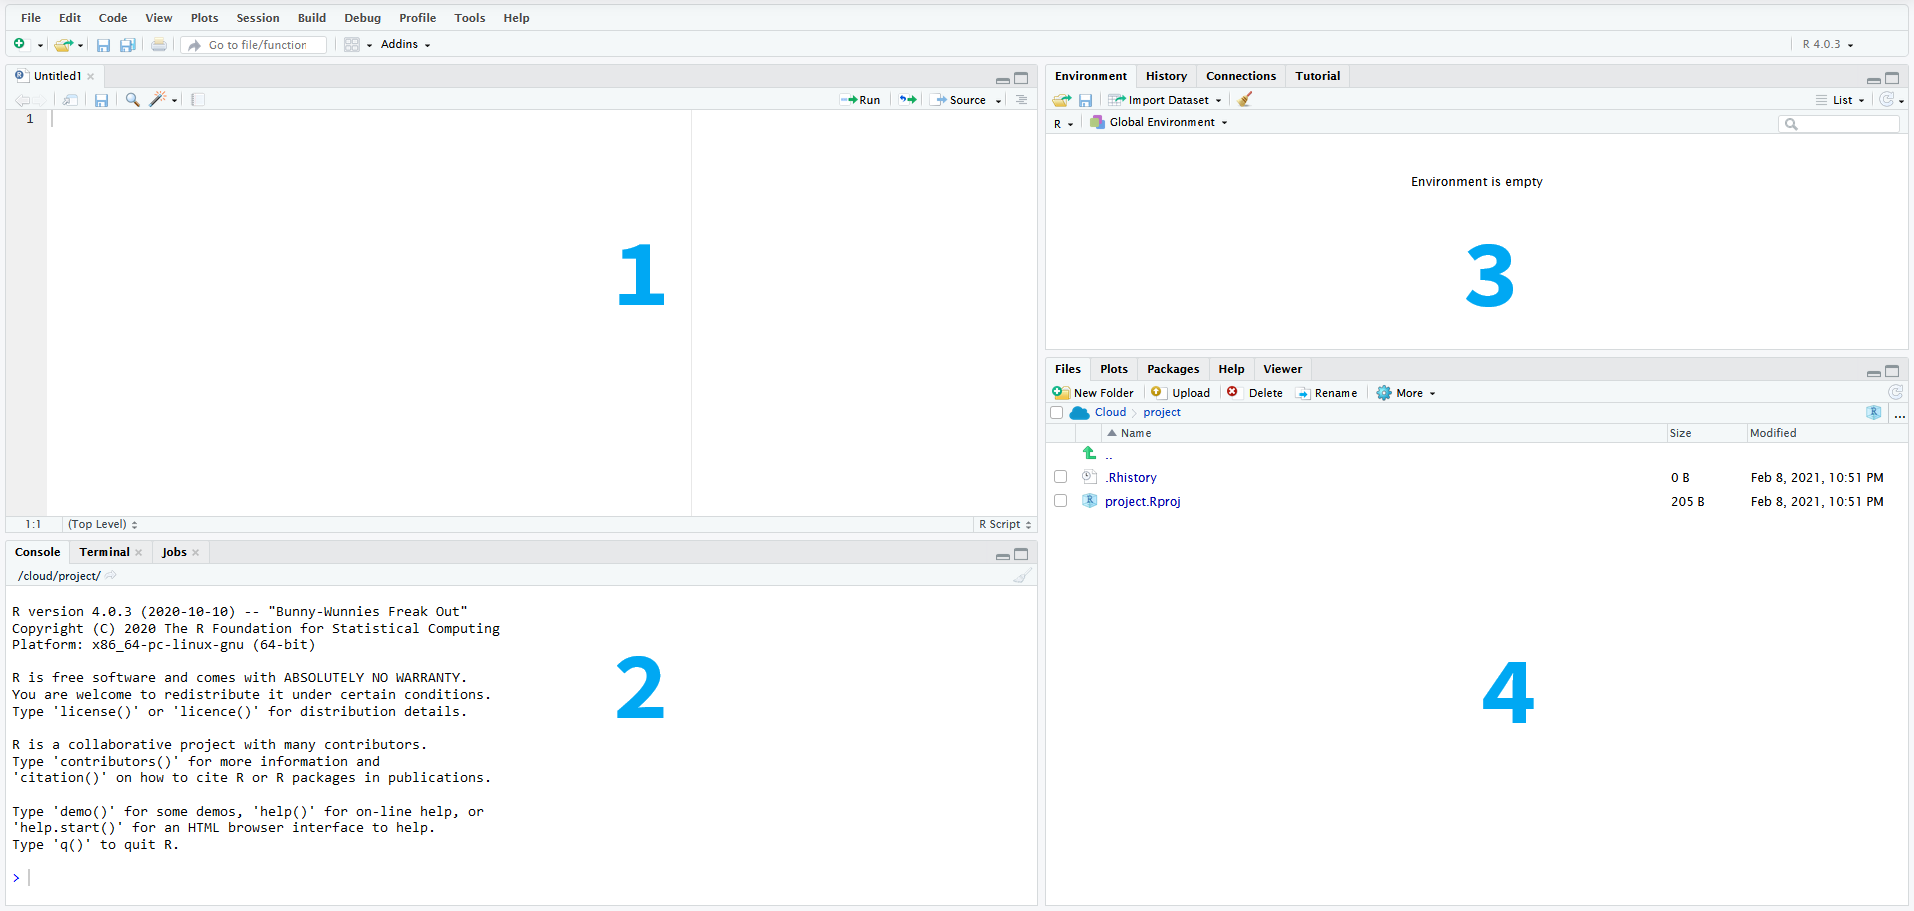
\includegraphics{figures/13-01_layout} 

}

\caption{RStudio felhasználói felület}\label{fig:unnamed-chunk-17}
\end{figure}

Az \textbf{\emph{(1) editor}} ablak szolgál a kód beírására, futtatására
és mentésére. A \textbf{\emph{(2) console}} ablakban jelenik meg a
lefuttatott kód és az eredmények. A jobb felső ablak \textbf{\emph{(3)
environment}} fülén láthatóak a memóriában tárolt adatállományok,
változók és felhasználói függvények. A \textbf{\emph{history}} fül
mutatja a korábban lefuttatott utasításokat. A jobb alsó ablak
\textbf{\emph{(4) files}} fülén az aktuális munkakönyvtárban levő
mappákat és fájlok találjuk, míg a \textbf{\emph{plot}} fülön az
elemzéseink során elkészített ábrák jelennek meg. A
\textbf{\emph{packages}} fülön frissíthetjük a meglévő r csomagokat és
telepíthetünk újakat. A \textbf{\emph{help}} fülön a különböző
függvények, parancsok leírását, és használatát találjuk meg. A
\texttt{Tools\ -\textgreater{}\ Global\ Options} menüpont végezhetjük el
az RStudio testreszabását. Így például beállíthatjuk az ablaktér
elrendezését (\emph{Pane layout}), vagy a színvilágot
(\emph{Appearance}), illetve azt hogy a kódok ne fussanak ki az ablakból
(\texttt{Code\ -\textgreater{}\ Editing\ -\textgreater{}\ Soft\ wrap\ R\ source\ files})

\hypertarget{projektmunka}{%
\subsection{Projekt alapú munka}\label{projektmunka}}

Bár nem kötelező, de javasolt, hogy az RStudio-ban projekt alapon
dolgozzunk, mivel így az összes -- az adott projekttel kapcsolatos fájlt
-- egy mappában tárolhatjuk. Új projekt beállítását a
\texttt{File-\textgreater{}New\ Project} menüben tehetjük meg, ahol a
saját gépünk egy könyvtárát kell kiválasztani, ahová az R scripteket, az
adat- és előzményfájlokat menti. Ezenkívül a
\texttt{Tools-\textgreater{}Global\ Options-\textgreater{}General}
menüpont alatt le kell tiltani a \emph{„Restore most recently opened
project at startup''} és a \emph{„Restore .RData ino workspace at
startup''} beállítást, valamint \emph{„Save workspace to .RData on
exit''} értékre be kell állítani a \emph{„Never''} értéket.

\begin{figure}

{\centering 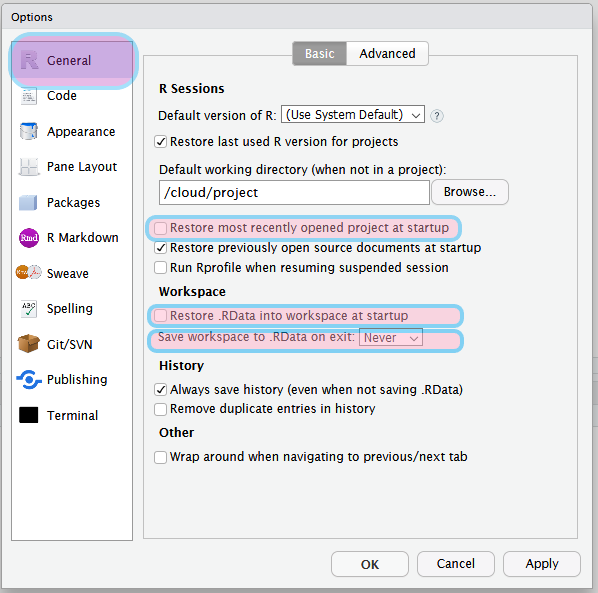
\includegraphics{figures/13-02_project_options} 

}

\caption{RStudio projekt beállítások}\label{fig:unnamed-chunk-18}
\end{figure}

A szükséges beállítások után a
\texttt{File\ -\textgreater{}\ New\ Project} menüben hozhatjuk létre a
projektet. Itt arra is lehetőségünk van, hogy kiválasszuk, hogy a
projektünket egy teljesen új könyvtárba, vagy egy meglévőbe kívánjuk
menteni, esetleg egy meglévő projekt új verzióját szeretnénk létrehozni.
Ha sikeresen létrehoztuk a projektet, az RStudio jobb felső sarkában
látnunk kell annak nevét.

\hypertarget{scriptek-szerkesztuxe9se-fuxfcggvuxe9nyek-hasznuxe1lata}{%
\subsection{Scriptek szerkesztése, függvények
használata}\label{scriptek-szerkesztuxe9se-fuxfcggvuxe9nyek-hasznuxe1lata}}

Új script a
\texttt{File\ -\textgreater{}\ New\ -\textgreater{}\ File\ -\textgreater{}\ R}
Script menüpontban hozható létre, mentésére a File-\textgreater Save
menüpontban egy korábbi script megnyitására
\texttt{File\ -\textgreater{}\ Open} menüpontban van lehetőségünk.
Script bármilyen szövegszerkesztővel írható és beilleszthető az editor
ablakba. A scripteket érdemes magyarázatokkal (kommentekkel) ellátni,
hogy a későbbiekben pontosan követhető legyen, hogy melyik parancs
segítségével pontosan milyen lépéseket hajtottunk végre. A
magyarázatokat vagy más néven kommenteket kettőskereszt (\texttt{\#})
karakterrel vezetjük be. A scriptbeli utasítások az azokat tartalmazó
sorokra állva vagy több sort kijelölve a Run feliratra kattintva vagy a
\texttt{Ctrl+Enter} billentyűparanccsal futtathatók le. A lefuttatott
parancsok és azok eredményei ezután a bal alsó sarokban lévő console
ablakban jelennek meg és ugyanitt kapunk hibaüzenetet is, ha valamilyen
hibát vétettünk a scriptben.

A munkafolyamat során létrehozott állományok (ábrák, fájlok) ebbe az ún.
munkakönyvtárba (\emph{working directory}) mentődnek. Az aktuális
munkakönyvtár neve, elérési útja a \texttt{getwd()} utasítással
jeleníthető meg. A könyvtárban található állományok listázására a
\texttt{list.files()} utasítással van lehetőségünk. Ha a korábbiaktól
eltérő munkakönyvtárat akarunk megadni, azt a \texttt{setwd()}
függvénnyel tehetjük meg, ahol a ()-ben az adott mappa elérési útját
kell megadnunk. Az elérési útban a meghajtó azonosítóját, majd a mappák,
almappák nevét vagy egy normál irányú perjel (\texttt{/}), vagy két
fordított perjel (\texttt{\textbackslash{}\textbackslash{}}) választja
el, mivel az elérési út karakterlánc, ezért azt idézőjelek vagy
aposztrófok közé kell tennünk. Az aktuális munkakönyvtárba beléphetünk a
jobb alsó ablak file lapján a
\texttt{„More\ -\textgreater{}\ Go\ To\ Working\ Directory”}
segítségével. Ugyanitt a \texttt{„Set\ Working\ Directory”}-val
munkakönyvtárnak állíthatjuk be az a mappát, amelyben épp benne vagyunk.

\begin{figure}

{\centering 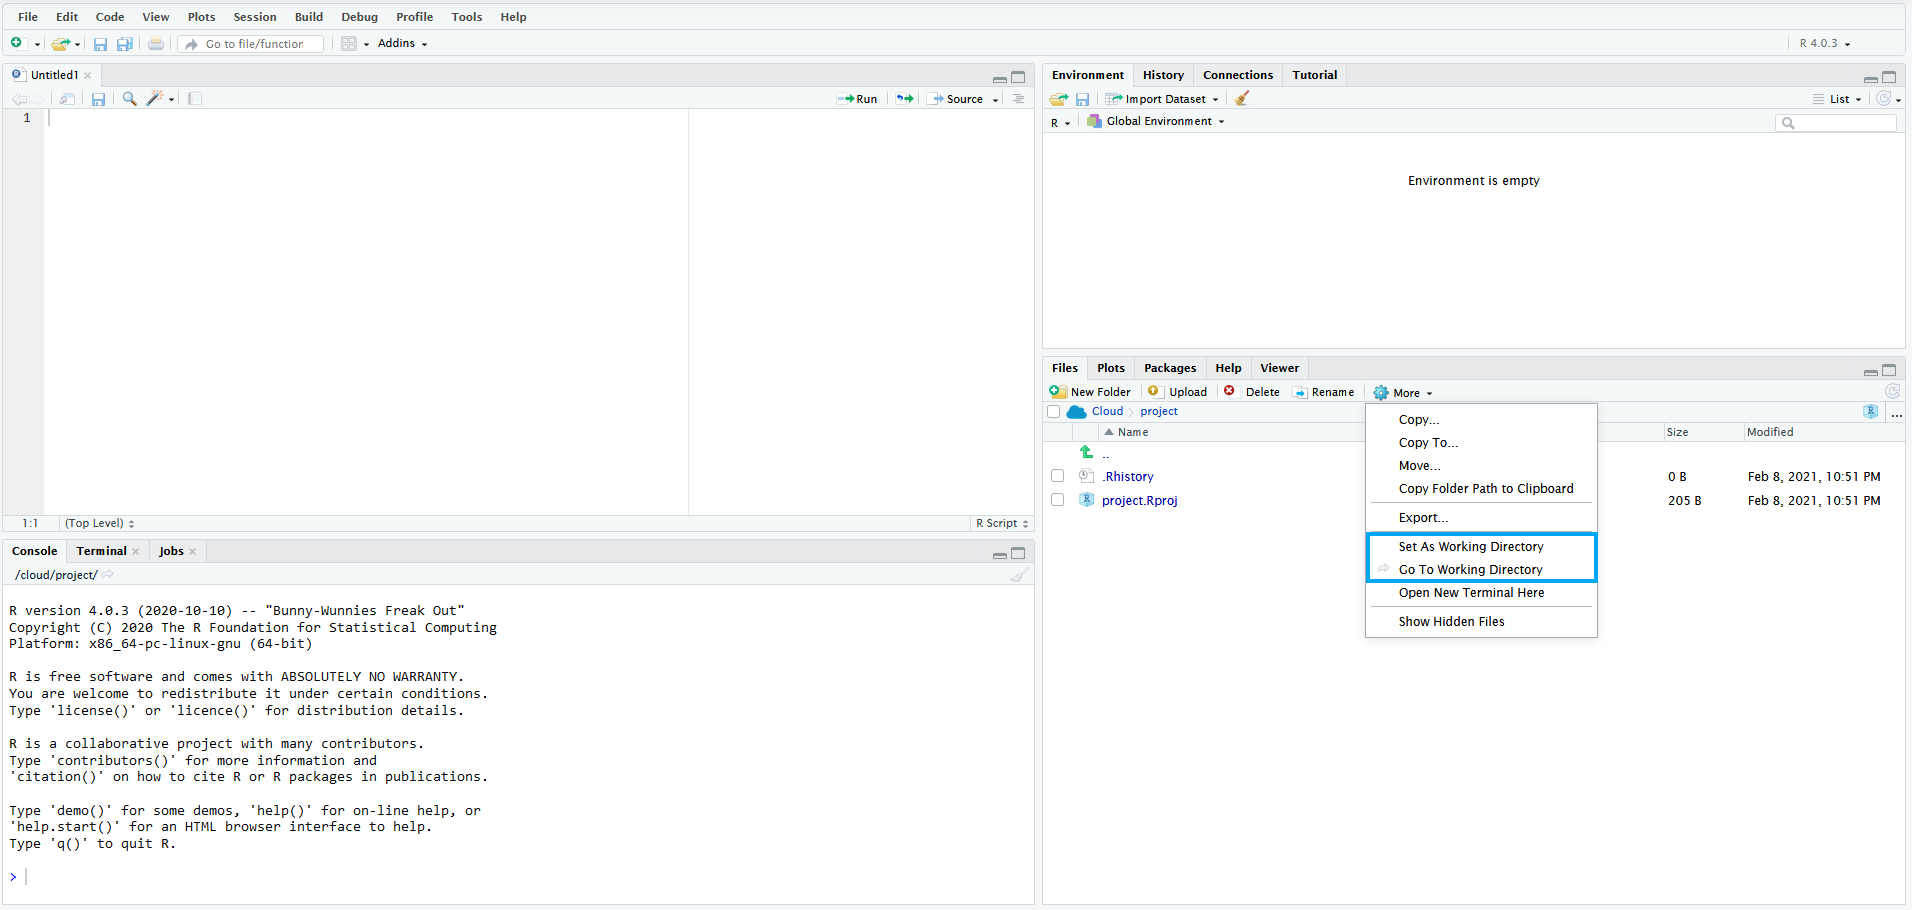
\includegraphics{figures/13-03_working_directory} 

}

\caption{Working directory beállítások}\label{fig:unnamed-chunk-19}
\end{figure}

A munkafolyamat befejezésére a \texttt{q()} vagy \texttt{quit()}
függvényel van lehetőségünk. A munkafolyamat során különböző
objektumokat hozunk létre, melyek az RStudio jobb felső ablakának
environment fülén jelennek meg, a mentett objektumokat a fent látható
seprű ikonra kattintva törölhetjük a memóriából. Az environment ablakra
érdemes úgy gondolni hogy ott jelennek meg a memóriában tárolt értékek.
Az R-ben objektumokkal dolgozunk, amik a teljesség igénye nélkül
lehetnek egyszerű szám vektortok, vagy akár komplex listák, illetve
függvények, ábrák.

Az RStudio jobb alsó ablakának plots fülén láthatjuk azon parancsok
eredményét, melyek kimenete valamilyen ábra. A packages fülnél a már
telepített és a letölthető kiegészítő csomagokat jeleníthetjük meg. A
help fülön a korábban említettek szerint a súgó érhető el. Az
RStudio-ban használható billentyűparancsok teljes listáját Alt+Shift+K
billentyűkombinációval tekinthetjük meg. Néhány gyakrabban használt,
hasznos billentyűparancs:

\begin{itemize}
\tightlist
\item
  \texttt{Ctrl+Enter}: futtassa a kódot az aktuális sorban
\item
  \texttt{Ctrl+Alt+B}: futtassa a kódot az elejétől az aktuális sorig
\item
  \texttt{Ctrl+Alt+E}: futtassa a kódot az aktuális sortól a forrásfájl
  végéig
\item
  \texttt{Ctrl+D}: törölje az aktuális sort
\end{itemize}

Az R-ben beépített \textbf{függvények (function)} állnak
rendelkezésünkre a számítások végrehajtására, emellett több
\textbf{csomag (package)} is letölthető, amelyek különböző függvényeket
tartalmaznak. A függvények a következőképpen épülnek fel:
\texttt{függvénynév(paraméter)}. Például tartalom képernyőre való
kiíratását a \texttt{print()} függvénnyel tehetjük, amelynek gömbölyű
zárójelekkel határolt részébe írhatjuk a megjelenítendő szöveget. A
\texttt{citation()} függvénnyel lekérdezhetjük az egyes beépített
csomagokra való hivatkozást is: a \texttt{citation(quanteda)} függvény a
quanteda csomag hivatkozását adja meg. Az R súgórendszere a
\texttt{help.start()} utasítással indítható el. Egy adott függvényre
vonatkozó súgórészlet a függvények neve elé kérdőjel írásával, vagy a
\texttt{help()} argumentumába a kérdéses függvény nevének beírásával
jeleníthető meg (pl.: \texttt{help(sum)}).

\hypertarget{packages}{%
\subsection{R csomagok}\label{packages}}

Az R-ben telepíthetők kiegészítő csomagok (packages), amelyek
alapértelmezetten el nem érhető algoritmusokat, függvényeket
tartalmaznak. A csomagok saját dokumentációval rendelkeznek, amelyeket
fel kell tüntetni a használatukkal készült publikációink
hivatkozáslistájában. A csomagok telepítésre több lehetőségünk is van:
használhatjuk a menüsor
\texttt{Tools\ -\textgreater{}\ Install\ Packages} menüpontját, vagy a
jobb alsó ablak \emph{Packages} fül Install menüpontját, illetve az
editor ablakban az \texttt{install.packages()} parancsot futtatva, ahol
a ()-be a telepíteni kívánt csomag nevét kell beírnunk (pl.:
\texttt{install.packages(dplyr)}).

\begin{figure}

{\centering 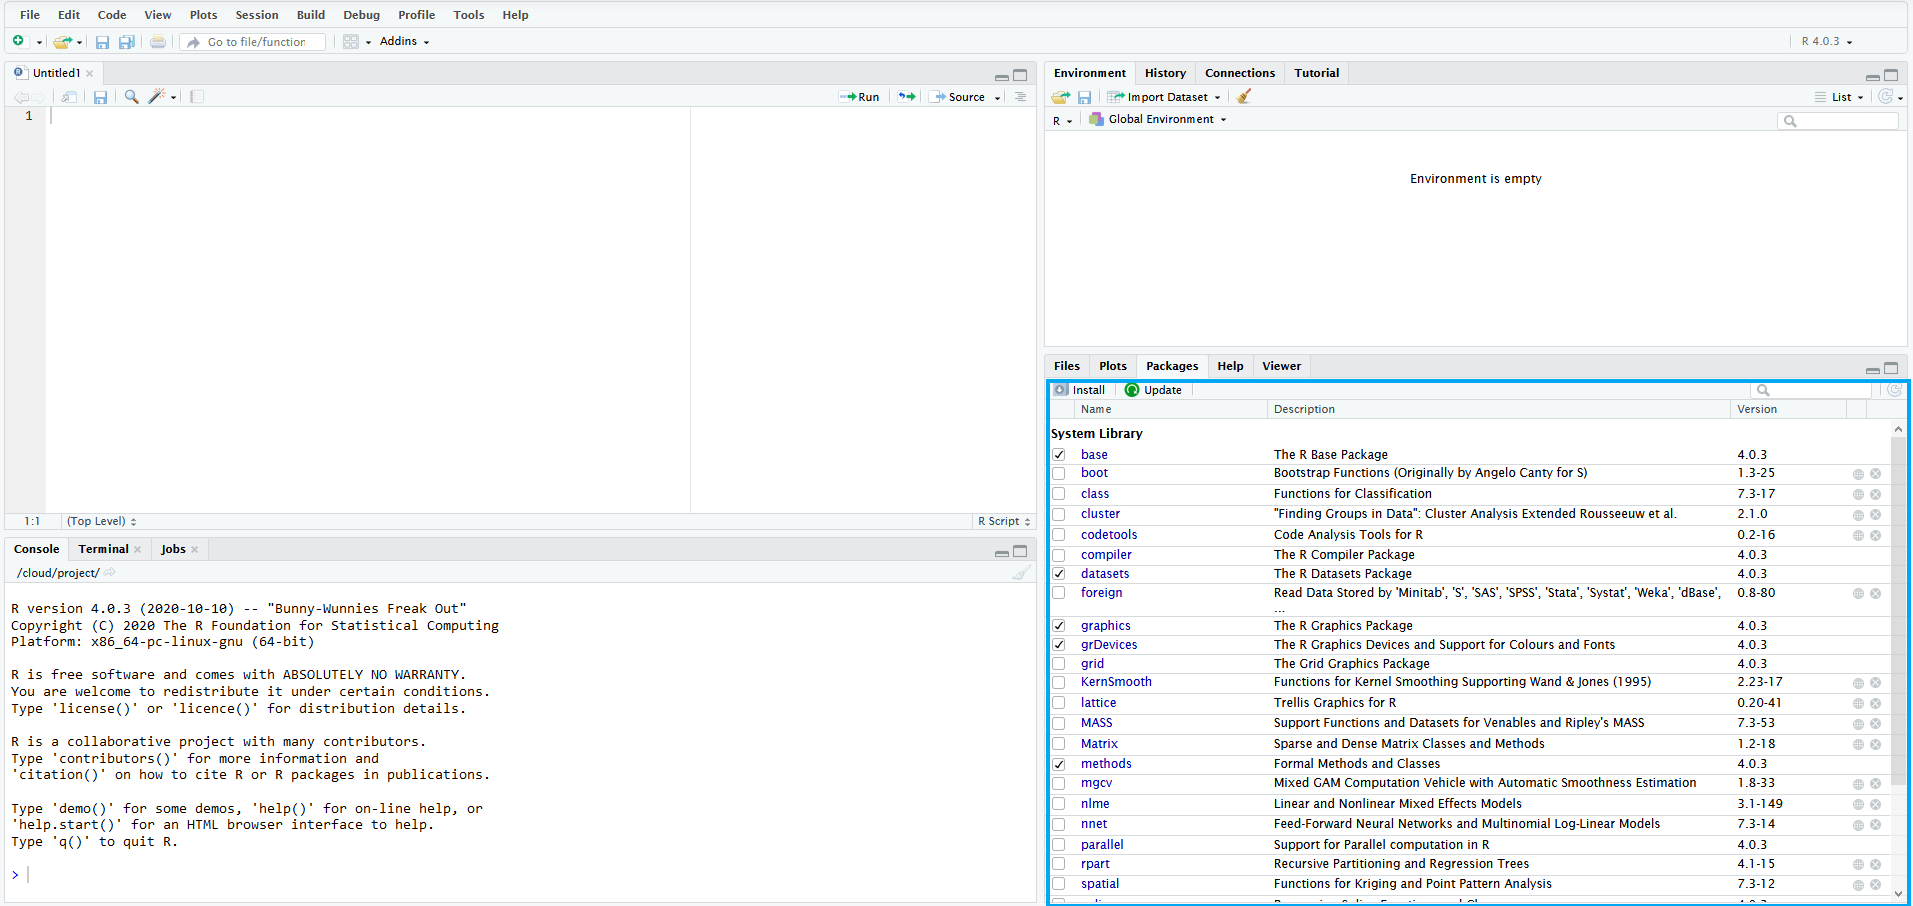
\includegraphics{figures/13-04_packages} 

}

\caption{Packages fül}\label{fig:unnamed-chunk-20}
\end{figure}

\hypertarget{objektumok-tuxe1roluxe1sa-uxe9rtuxe9kaduxe1s}{%
\subsection{Objektumok tárolása,
értékadás}\label{objektumok-tuxe1roluxe1sa-uxe9rtuxe9kaduxe1s}}

Az objektumok lehetnek például \emph{vektorok}, \emph{mátrixok}
(matrix), \emph{tömbök} (array), \emph{adat táblák} (data frame).
Értékadás nélkül az R csak megjeleníti a műveletek eredményét, de nem
tárolja el azokat. Az eredmények eltárolásához azokat egy objektumba
kell elmentenünk. Ehhez meg kell adnunk az objektum nevét majd az
\texttt{\textless{}-} után adjuk meg annak értékét:
\texttt{a\ \textless{}-\ 12\ +\ 3}.Futtatás után az environments fülön
megjelenik az a objektum, melynek értéke \texttt{15}. Az objektumok
elnevezésénél figyelnünk kell arra, hogy az R különbséget tesz a kis és
nagybetűk között, valamint, hogy az ugyanolyan nevű objektumokat kérdés
nélkül felülírja és ezt a felülírást nem lehet visszavonni.

\hypertarget{vektorok}{%
\subsection{Vektorok}\label{vektorok}}

Az R-ben kétféle típusú vektort különböztetünk meg:

\begin{itemize}
\tightlist
\item
  egyedüli vektor (atomic vector)
\item
  lista (list)
\end{itemize}

Az egyedüli vektornak hat típusa van, \textbf{logikai} (logical),
\textbf{egész szám} (integer), \textbf{természetes szám} (double),
\textbf{karakter} (character), \textbf{komplex szám} (complex) és
\textbf{nyers adat} (raw). A leggyakrabban valamilyen numerikus, logikai
vagy karakter vektorral használjuk. Az egyedüli vektorok onnan kapták a
nevüket hogy csak egy féle adattípust tudnak tárolni. A listák ezzel
szemben gyakorlatilag bármit tudnak tárolni, akár több listát is
egybeágyazhatunk.

A vektorok és listák azok az építőelemek amikből felépülnek az R
objektumaink. Több érték vagy azonos típusú objektum összefűzését a
\texttt{c()} függvénnyel végezhetjük el. A lenti példában három
különböző objektumot kreálunk, egy numerikusat, egy karaktert és egy
logikait. A karakter vektorban az elemeket időzőjellel és vesszővel
szeparáljuk. A logikai vektor csak \texttt{TRUE}, illetve \texttt{FALSE}
értékeket tartalmazhat.

\begin{Shaded}
\begin{Highlighting}[]
\NormalTok{numerikus }\OtherTok{\textless{}{-}} \FunctionTok{c}\NormalTok{(}\DecValTok{1}\NormalTok{,}\DecValTok{2}\NormalTok{,}\DecValTok{3}\NormalTok{,}\DecValTok{4}\NormalTok{,}\DecValTok{5}\NormalTok{)}

\NormalTok{karakter }\OtherTok{\textless{}{-}} \FunctionTok{c}\NormalTok{(}\StringTok{"kutya"}\NormalTok{,}\StringTok{"macska"}\NormalTok{,}\StringTok{"ló"}\NormalTok{)}

\NormalTok{logikai }\OtherTok{\textless{}{-}} \FunctionTok{c}\NormalTok{(}\ConstantTok{TRUE}\NormalTok{, }\ConstantTok{TRUE}\NormalTok{, }\ConstantTok{FALSE}\NormalTok{)}
\end{Highlighting}
\end{Shaded}

A létrehozott vektorokkal különböző műveleteket végezhetünk el, például
összeadhatjuk numerikus vektorainkat. Ebben az esetben az első vektor
első eleme a második vektor első eleméhez adódik.

\begin{Shaded}
\begin{Highlighting}[]
\FunctionTok{c}\NormalTok{(}\DecValTok{1}\SpecialCharTok{:}\DecValTok{4}\NormalTok{) }\SpecialCharTok{+} \FunctionTok{c}\NormalTok{(}\DecValTok{10}\NormalTok{,}\DecValTok{20}\NormalTok{,}\DecValTok{30}\NormalTok{,}\DecValTok{40}\NormalTok{)}
\end{Highlighting}
\end{Shaded}

\begin{verbatim}
## [1] 11 22 33 44
\end{verbatim}

A karaktervektorokat összefűzhetjük egymással. Itt egy új objektumot is
létrehoztunk, a jobb felső ablakban, az environment fülön láthatjuk,
hogy a létrejött karakter\_kombinalt objektum egy négy elemű
(hosszúságú) karaktervektor (\texttt{chr\ {[}1:4{]}}), melynek elemei a
\texttt{"kutya","macska","ló","nyúl"}. Az objektumként tárolt vektorok
tartalmát a lefuttatva írathatjuk ki a console ablakba. Habár van
\texttt{print()} függvény az R-ben, azt ilyenkor nem szükséges
használni.

\begin{Shaded}
\begin{Highlighting}[]
\NormalTok{karakter1 }\OtherTok{\textless{}{-}} \FunctionTok{c}\NormalTok{(}\StringTok{"kutya"}\NormalTok{,}\StringTok{"macska"}\NormalTok{,}\StringTok{"ló"}\NormalTok{)}
\NormalTok{karakter2 }\OtherTok{\textless{}{-}}\FunctionTok{c}\NormalTok{(}\StringTok{"nyúl"}\NormalTok{)}

\NormalTok{karakter\_kombinalt }\OtherTok{\textless{}{-}}\FunctionTok{c}\NormalTok{(karakter1, karakter2)}

\NormalTok{karakter\_kombinalt}
\end{Highlighting}
\end{Shaded}

\begin{verbatim}
## [1] "kutya"  "macska" "ló"     "nyúl"
\end{verbatim}

Ha egy vektorról szeretnénk megtudni, hogy milyen típusú azt a
\texttt{typeof()} vagy a \texttt{class()} paranccsal tehetjük meg, ahol
()-ben az adott objektumként tárolt vektor nevét kell megadnunk:
\texttt{typeof(karakter1)}. A vektor hosszúságát (benne tárolt elemek
száma vektorok esetén) a \texttt{lenght()} függvénnyel tudhatjuk meg.

\begin{Shaded}
\begin{Highlighting}[]
\FunctionTok{typeof}\NormalTok{(karakter1)}
\end{Highlighting}
\end{Shaded}

\begin{verbatim}
## [1] "character"
\end{verbatim}

\begin{Shaded}
\begin{Highlighting}[]
\FunctionTok{length}\NormalTok{(karakter1)}
\end{Highlighting}
\end{Shaded}

\begin{verbatim}
## [1] 3
\end{verbatim}

\hypertarget{faktorok}{%
\subsection{Faktorok}\label{faktorok}}

A faktorok a kategórikus adatok tárolására szolgálnak. Faktor típusú
változó a \texttt{factor()} függvénnyel hozható létre. A faktor
szintjeit (igen, semleges, nem), a \texttt{levels()} függvénnyel
kaphatjuk meg míg az adatok címkéit (tehát a kapott válaszok száma), a
\texttt{labels()} paranccsal érhetjük el.

\begin{Shaded}
\begin{Highlighting}[]
\NormalTok{survey\_response }\OtherTok{\textless{}{-}} \FunctionTok{factor}\NormalTok{(}\FunctionTok{c}\NormalTok{(}\StringTok{"igen"}\NormalTok{, }\StringTok{"semleges"}\NormalTok{, }\StringTok{"nem"}\NormalTok{, }\StringTok{"semleges"}\NormalTok{, }\StringTok{"nem"}\NormalTok{, }\StringTok{"nem"}\NormalTok{, }\StringTok{"igen"}\NormalTok{), }\AttributeTok{ordered =} \ConstantTok{TRUE}\NormalTok{)}


\FunctionTok{levels}\NormalTok{(survey\_response)}
\end{Highlighting}
\end{Shaded}

\begin{verbatim}
## [1] "igen"     "nem"      "semleges"
\end{verbatim}

\begin{Shaded}
\begin{Highlighting}[]
\FunctionTok{labels}\NormalTok{(survey\_response)}
\end{Highlighting}
\end{Shaded}

\begin{verbatim}
## [1] "1" "2" "3" "4" "5" "6" "7"
\end{verbatim}

\hypertarget{data-frame}{%
\subsection{Data frame}\label{data-frame}}

Az adat táblák (data frame) a statisztikai és adatelemzési folyamatok
egyik leggyakrabban használt adattárolási formája. Amikor lehetséges
akkor a `hosszú' formátumban használjuk (az R közösség a `tidy' jelzővel
illeti), aholtéglalap alakú adatszerkezetek, ahol minden sor egy
megfigyelés és minden oszlop egy változó {[}TIDY CITATION{]}. Egy data
frame többféle típusú adatot tartalmazhat. A data frame-k különféle
oszlopokból állhatnak, amelyek különféle típusú adatokat
tartalmazhatnak, de egy oszlop csak egy típusú adatból állhat. A lent
bemutatott data frame 7 megfigyelést és 4 féle változót tartalmaz (id,
country, pop, continent).

\begin{verbatim}
##   id      orszag nepesseg     kontinens
## 1  1    Thailand     68.7          Asia
## 2  2      Norway      5.2        Europe
## 3  3 North Korea     24.0          Asia
## 4  4      Canada     47.8 North America
## 5  5    Slovenia      2.0        Europe
## 6  6      France     63.6        Europe
## 7  7   Venezuela     31.6 South America
\end{verbatim}

A data frame-be rendezett adatokhoz különböző módon férhetünk hozzá,
például a data frame nevének majd {[}{]}-ben a kívánt sor megadásával,
kiírathatjuk a console ablakba annak tetszőleges sorát ás oszlopát:
\texttt{orszag\_adatok{[}1,\ 1{]}}. Az R több különböző módot kínál a
data frame sorainak és oszlopainak eléréséhez. A \texttt{{[}} általános
használata: \texttt{data\_frame{[}sor,\ oszlop{]}}. Egy másik megoldás a
\texttt{\$} haszálata: \texttt{data\_frame\$oszlop}.

\begin{Shaded}
\begin{Highlighting}[]
\NormalTok{orszag\_adatok[}\DecValTok{1}\NormalTok{, }\DecValTok{4}\NormalTok{]}
\end{Highlighting}
\end{Shaded}

\begin{verbatim}
## [1] Asia
## Levels: Asia Europe North America South America
\end{verbatim}

\begin{Shaded}
\begin{Highlighting}[]
\NormalTok{orszag\_adatok}\SpecialCharTok{$}\NormalTok{orszag}
\end{Highlighting}
\end{Shaded}

\begin{verbatim}
## [1] "Thailand"    "Norway"      "North Korea" "Canada"      "Slovenia"   
## [6] "France"      "Venezuela"
\end{verbatim}

\hypertarget{vizualizuxe1ciuxf3}{%
\section{Vizualizáció}\label{vizualizuxe1ciuxf3}}

\begin{Shaded}
\begin{Highlighting}[]
\FunctionTok{library}\NormalTok{(ggplot2)}
\FunctionTok{library}\NormalTok{(gapminder)}
\end{Highlighting}
\end{Shaded}

Az elemzéseinkhez használt data frame adatainak alapján a
\texttt{ggplot2} csomag segítségével lehetőségünk van különböző
vizualizációk készítésére is.

A \texttt{ggplot2} használata során különböző témákat alkalmazhatunk,
melyek részletes leírása megtalálható:
\url{https://ggplot2.tidyverse.org/reference/ggtheme.html}

Abban az esetben, ha nem választunk témát, a \texttt{ggplot2} a
következő ábrán is látható alaptémát használja. Ha például a szürke
helyett fehér hátteret szeretnénk, alkalmazhatjuk a
\texttt{theme\_minmal()}parancsot. Szintén gyakran alkalmazott ábra alap
a \texttt{thema\_bw()}, ami az előzőtől az ábra keretezésében
különbözik. Ha fehér alapon, de a beosztások vonalait feketén szeretnénk
megjeleníteni, alkalmazhatjuk a \texttt{theme\_linedraw()} függvényt, a
\texttt{theme\_void()} segítségével pedig egy fehér alapon,
beosztásoktól mentes alapot kapunk, a \texttt{theme\_dark()} pedig sötét
hátteret eredményez. A \texttt{theme\_classic()} segítségével az x és y
tengelyt jeleníthetjük meg fehér alapon.

Egy ábra készítésének alapja mindig a használni kívánt adatkészlet
beolvasása, illetve az ábrázolni kiíván változtót vagy változók
megadása.

Ezt követi a megfelelő alakzat kiválasztása, attól függően például, hogy
eloszlást, változást, adatok közötti kapcsolatot, vagy elétéseket
akarunk ábrázolni. A \texttt{geom} az a geometriai objektum, a mit a
diagram az adatok megjelenítésére használ. A\texttt{gglpot2} több mint
40 féle alakzat alkalmazására ad lehetőséget, ezek közül néhány
gyakoribbat mutatunk be az alábbiakban. Az alakzatokról részletes
leírása található például az alábbi linken:
\url{https://r4ds.had.co.nz/data-visualisation.html}

A következőkben a már korábban is használt \texttt{gapminder} adatok
segítségével, személetetjük az adatok vizualizálásának alapjait. Először
egyszerű alapbeállítások mellett egy histogram típusú vizualizációt
készítünk.

\begin{Shaded}
\begin{Highlighting}[]
\FunctionTok{ggplot}\NormalTok{(}
  \AttributeTok{data =}\NormalTok{ gapminder, }
  \AttributeTok{mapping =} \FunctionTok{aes}\NormalTok{(}\AttributeTok{x =}\NormalTok{ gdpPercap)}
\NormalTok{) }\SpecialCharTok{+} 
  \FunctionTok{geom\_histogram}\NormalTok{() }
\end{Highlighting}
\end{Shaded}

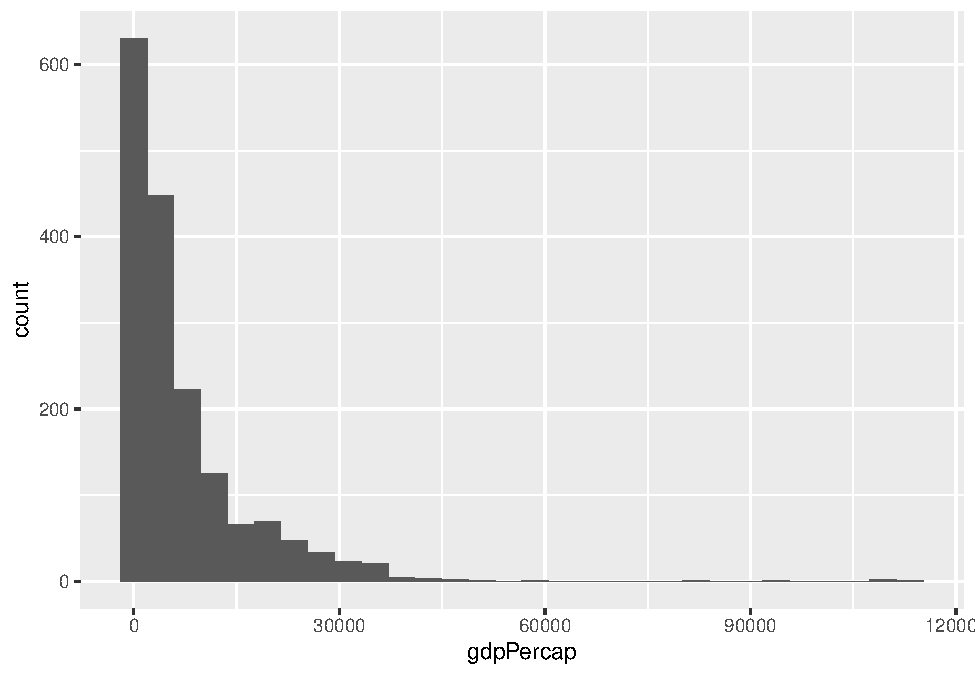
\includegraphics{_main_files/figure-latex/unnamed-chunk-30-1.pdf}

Lehetőségünk van arra, hogy az alakzat színét megváltoztatássuk. A
használható színek és színkódok megtalálhatóak a \texttt{ggplot2}
leírásában: \url{https://ggplot2-book.org/scale-colour.html}

\begin{Shaded}
\begin{Highlighting}[]
\FunctionTok{ggplot}\NormalTok{(}
  \AttributeTok{data =}\NormalTok{ gapminder,}
  \AttributeTok{mapping =} \FunctionTok{aes}\NormalTok{(}\AttributeTok{x =}\NormalTok{ gdpPercap)}
\NormalTok{) }\SpecialCharTok{+}
  \FunctionTok{geom\_histogram}\NormalTok{(}\AttributeTok{fill =} \StringTok{"yellow"}\NormalTok{, }\AttributeTok{colour =} \StringTok{"green"}\NormalTok{) }
\end{Highlighting}
\end{Shaded}

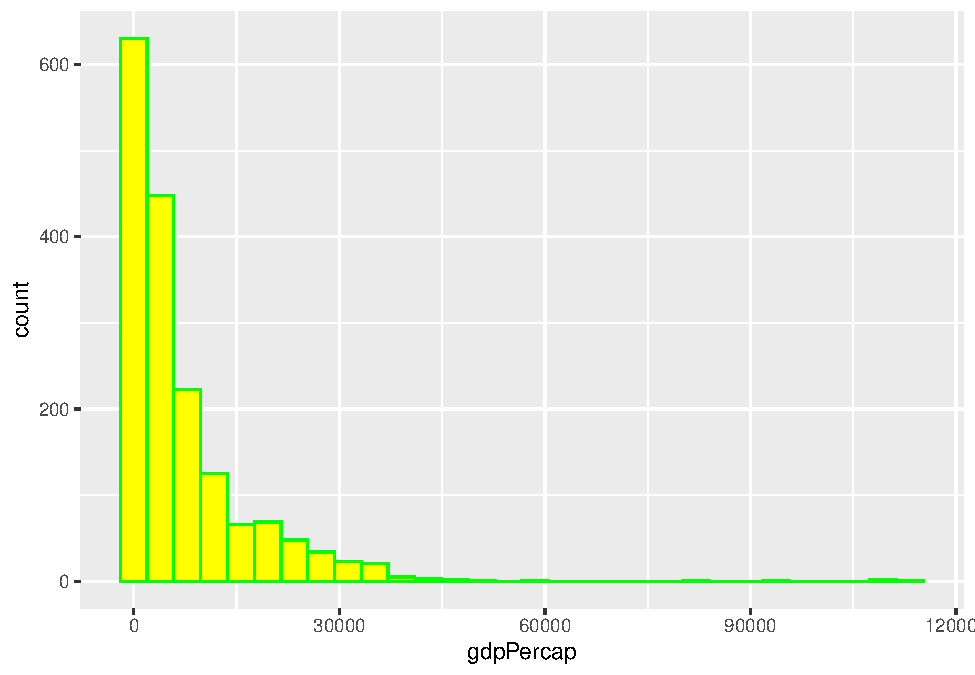
\includegraphics{_main_files/figure-latex/unnamed-chunk-31-1.pdf}

Meghatározhatjuk külön-külön a histogram x és y tengelyén ábrázolni
kívánt adatokat és választhatjuk azok pontszerű ábrázolását is.

\begin{Shaded}
\begin{Highlighting}[]
\FunctionTok{ggplot}\NormalTok{(}
  \AttributeTok{data =}\NormalTok{ gapminder,}
  \AttributeTok{mapping =} \FunctionTok{aes}\NormalTok{(}
    \AttributeTok{x =}\NormalTok{ gdpPercap,}
    \AttributeTok{y =}\NormalTok{ lifeExp}
\NormalTok{  )}
\NormalTok{) }\SpecialCharTok{+}
  \FunctionTok{geom\_point}\NormalTok{() }
\end{Highlighting}
\end{Shaded}

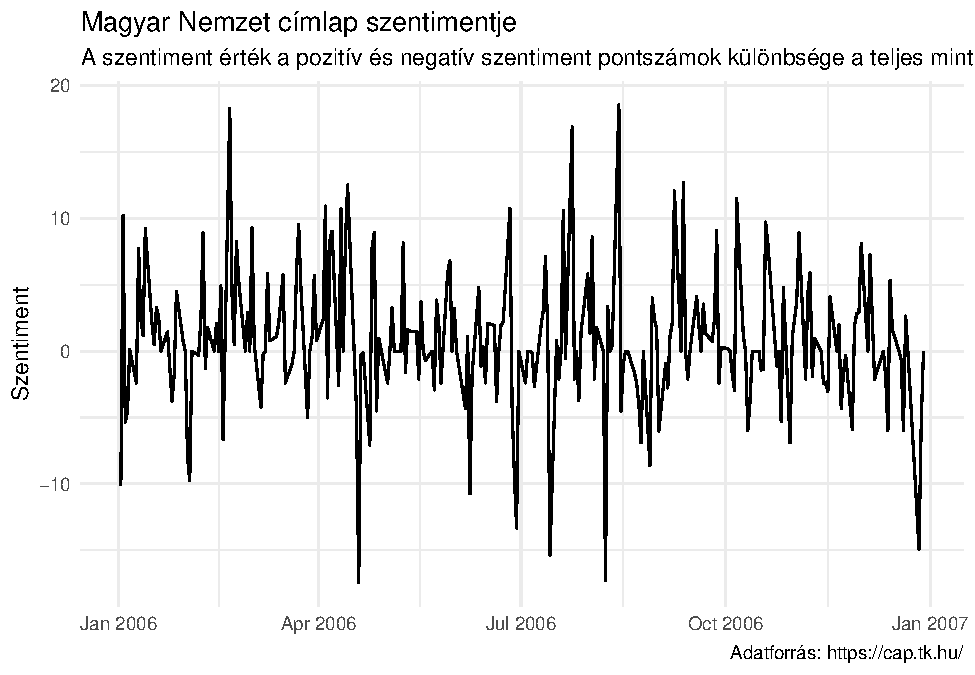
\includegraphics{_main_files/figure-latex/unnamed-chunk-32-1.pdf}

Ahogy az előzőekben, itt is megváltoztathatjuk az ábra színét.

\begin{Shaded}
\begin{Highlighting}[]
\FunctionTok{ggplot}\NormalTok{(}
  \AttributeTok{data =}\NormalTok{ gapminder,}
  \AttributeTok{mapping =} \FunctionTok{aes}\NormalTok{(}
    \AttributeTok{x =}\NormalTok{ gdpPercap,}
    \AttributeTok{y =}\NormalTok{ lifeExp}
\NormalTok{  )}
\NormalTok{) }\SpecialCharTok{+}
  \FunctionTok{geom\_point}\NormalTok{(}\AttributeTok{colour =} \StringTok{"blue"}\NormalTok{)}
\end{Highlighting}
\end{Shaded}

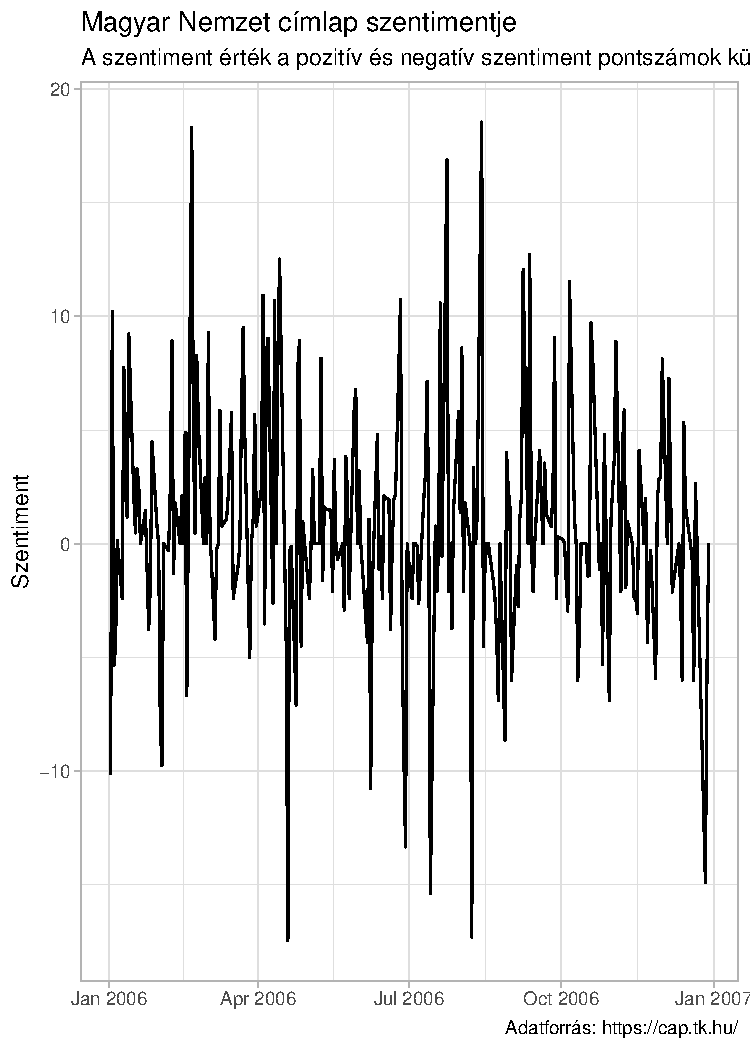
\includegraphics{_main_files/figure-latex/unnamed-chunk-33-1.pdf}

Az fenti script kibővítésével az egyes kontinensek adatait különböző
színnel ábrázolhatjuk, az x és y tengelyt elnevezhetjük, a histogramnak
címet és alcímet adhatunk, illetve az adataink forrását is
feltüntethetjük az alábbi módon:

\begin{Shaded}
\begin{Highlighting}[]
\FunctionTok{ggplot}\NormalTok{(}
  \AttributeTok{data =}\NormalTok{ gapminder,}
  \AttributeTok{mapping =} \FunctionTok{aes}\NormalTok{(}
    \AttributeTok{x =}\NormalTok{ gdpPercap,}
    \AttributeTok{y =}\NormalTok{ lifeExp,}
    \AttributeTok{color =}\NormalTok{ continent}
\NormalTok{  )}
\NormalTok{) }\SpecialCharTok{+} 
  \FunctionTok{geom\_point}\NormalTok{() }\SpecialCharTok{+}
  \FunctionTok{labs}\NormalTok{(}
    \AttributeTok{x =} \StringTok{"GDP per capita (log $)"}\NormalTok{, }
    \AttributeTok{y =} \StringTok{"Life expectancy"}\NormalTok{,}
    \AttributeTok{title =} \StringTok{"Connection between GDP and Life expectancy"}\NormalTok{,}
    \AttributeTok{subtitle =} \StringTok{"Points are country{-}years"}\NormalTok{,}
    \AttributeTok{caption =} \StringTok{"Source: Gapminder dataset"}
\NormalTok{  )}
\end{Highlighting}
\end{Shaded}

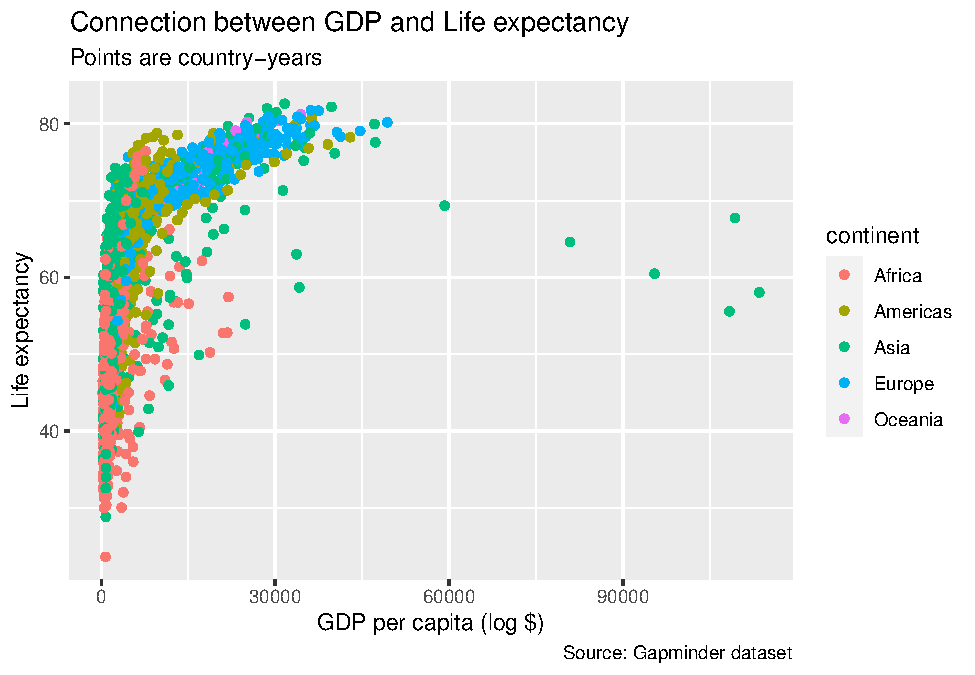
\includegraphics{_main_files/figure-latex/unnamed-chunk-34-1.pdf}

Az ábrán található feliratok méretének, betűtípusának és betűszínének
megválasztásra is lehetőségünk van.

\begin{Shaded}
\begin{Highlighting}[]
\FunctionTok{ggplot}\NormalTok{(}
  \AttributeTok{data =}\NormalTok{ gapminder,}
  \AttributeTok{mapping =} \FunctionTok{aes}\NormalTok{(}
    \AttributeTok{x =}\NormalTok{ gdpPercap,}
    \AttributeTok{y =}\NormalTok{ lifeExp,}
    \AttributeTok{color =}\NormalTok{ continent}
\NormalTok{  )}
\NormalTok{) }\SpecialCharTok{+} 
  \FunctionTok{geom\_point}\NormalTok{() }\SpecialCharTok{+}
  \FunctionTok{labs}\NormalTok{(}
    \AttributeTok{x =} \StringTok{"GDP per capita (log $)"}\NormalTok{, }
    \AttributeTok{y =} \StringTok{"Life expectancy"}\NormalTok{,}
    \AttributeTok{title =} \StringTok{"Connection between GDP and Life expectancy"}\NormalTok{,}
    \AttributeTok{subtitle =} \StringTok{"Points are country{-}years"}\NormalTok{,}
    \AttributeTok{caption =} \StringTok{"Source: Gapminder dataset"}
\NormalTok{  ) }\SpecialCharTok{+}
  \FunctionTok{theme}\NormalTok{(}\AttributeTok{plot.title =} \FunctionTok{element\_text}\NormalTok{(}
    \AttributeTok{size =} \DecValTok{12}\NormalTok{, }
    \AttributeTok{colour =} \StringTok{"red"}
\NormalTok{  ))}
\end{Highlighting}
\end{Shaded}

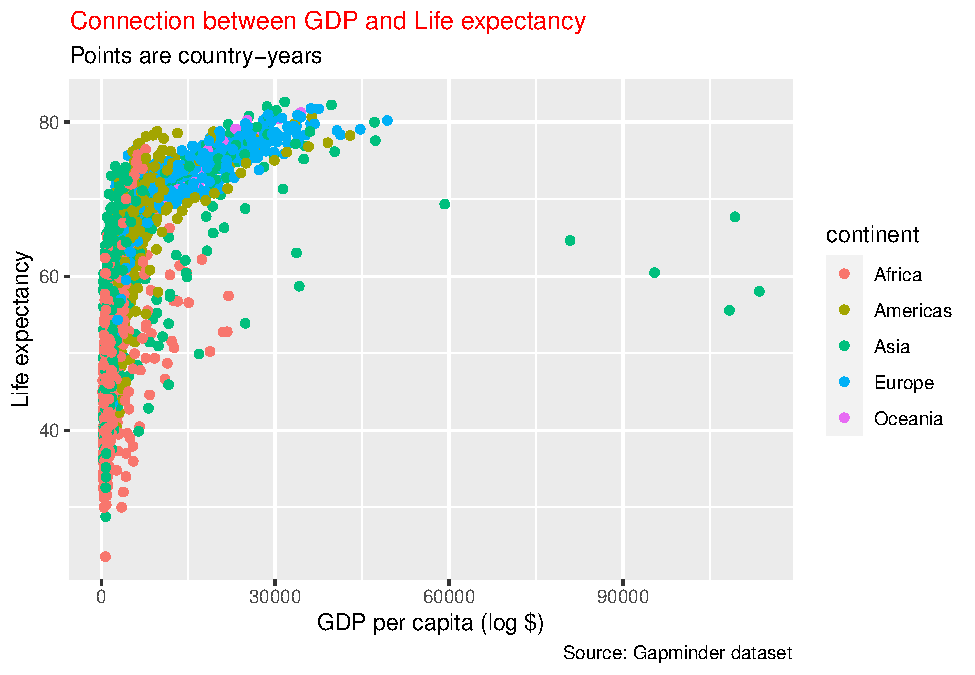
\includegraphics{_main_files/figure-latex/unnamed-chunk-35-1.pdf}

Készíthetünk oszlopdiagramot is, amit a \texttt{ggplot2} diamonds
adatkészletén személtetünk

\begin{Shaded}
\begin{Highlighting}[]
\FunctionTok{ggplot}\NormalTok{(}\AttributeTok{data =}\NormalTok{ diamonds) }\SpecialCharTok{+}
  \FunctionTok{geom\_bar}\NormalTok{(}\AttributeTok{mapping =} \FunctionTok{aes}\NormalTok{(}\AttributeTok{x =}\NormalTok{ cut))}
\end{Highlighting}
\end{Shaded}

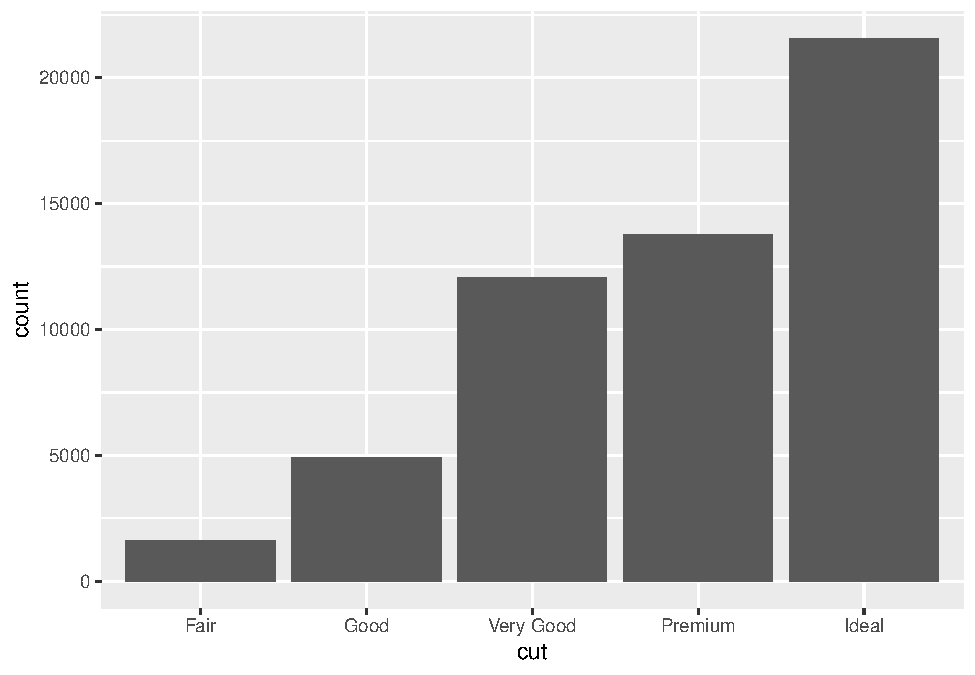
\includegraphics{_main_files/figure-latex/unnamed-chunk-36-1.pdf}

Itt is lehetőségünk van arra, hogy a diagram színét megváltoztassuk.

\begin{Shaded}
\begin{Highlighting}[]
\FunctionTok{ggplot}\NormalTok{(}\AttributeTok{data =}\NormalTok{ diamonds) }\SpecialCharTok{+}
  \FunctionTok{geom\_bar}\NormalTok{(}\AttributeTok{mapping =} \FunctionTok{aes}\NormalTok{(}\AttributeTok{x =}\NormalTok{ cut), }\AttributeTok{fill =} \StringTok{"darkgreen"}\NormalTok{)}
\end{Highlighting}
\end{Shaded}

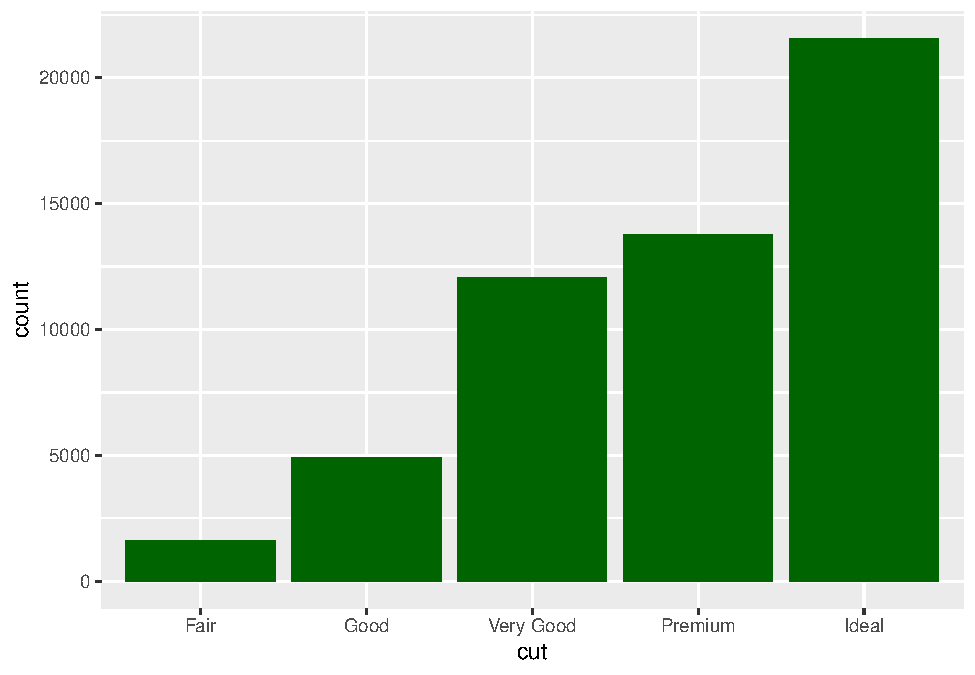
\includegraphics{_main_files/figure-latex/unnamed-chunk-37-1.pdf}

De arra is lehetőségünk van, hogy az egyes oszlopok eltérő színűek
legyenek.

\begin{Shaded}
\begin{Highlighting}[]
\FunctionTok{ggplot}\NormalTok{(}\AttributeTok{data =}\NormalTok{ diamonds) }\SpecialCharTok{+}
  \FunctionTok{geom\_bar}\NormalTok{(}\AttributeTok{mapping =} \FunctionTok{aes}\NormalTok{(}\AttributeTok{x =}\NormalTok{ cut, }\AttributeTok{fill =}\NormalTok{ cut))}
\end{Highlighting}
\end{Shaded}

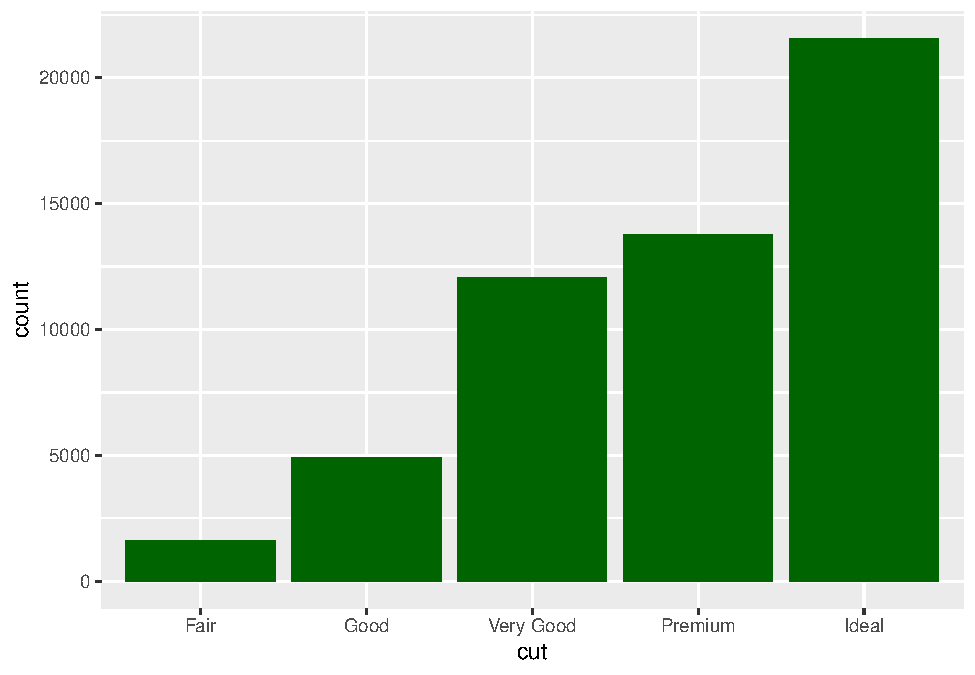
\includegraphics{_main_files/figure-latex/unnamed-chunk-38-1.pdf} Arra
is van lehetőségünk, hogy egyszerre több változót is ábrázoljunk.

\begin{Shaded}
\begin{Highlighting}[]
\FunctionTok{ggplot}\NormalTok{(}\AttributeTok{data =}\NormalTok{ diamonds) }\SpecialCharTok{+}
  \FunctionTok{geom\_bar}\NormalTok{(}\AttributeTok{mapping =} \FunctionTok{aes}\NormalTok{(}\AttributeTok{x =}\NormalTok{ cut, }\AttributeTok{fill =}\NormalTok{ clarity))}
\end{Highlighting}
\end{Shaded}

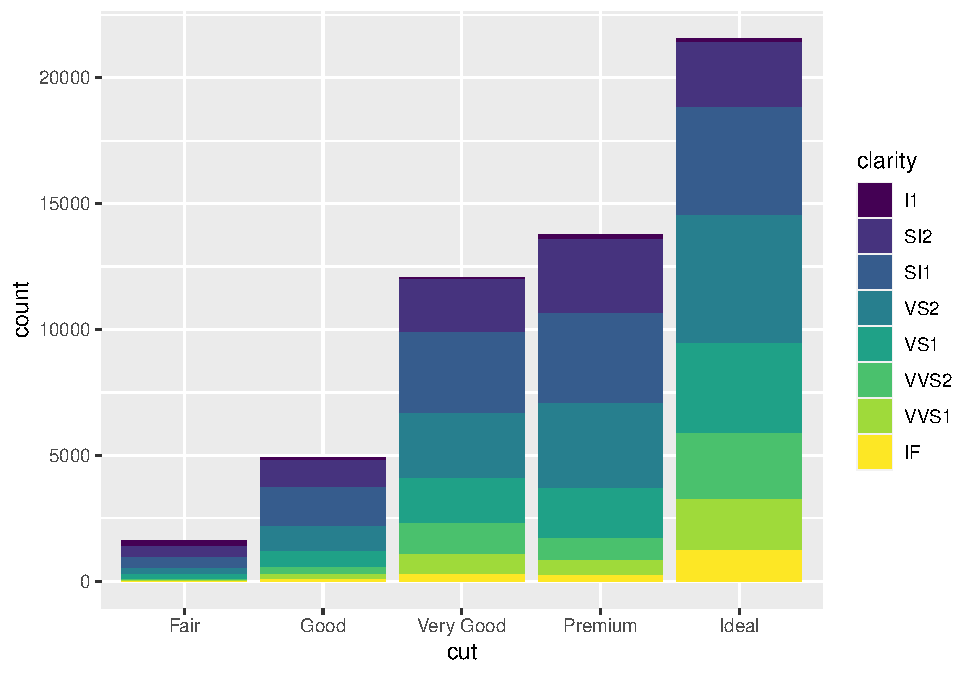
\includegraphics{_main_files/figure-latex/unnamed-chunk-39-1.pdf}

Arra ggplot2 segítségével arra is lehetőségünk van, hogy csv-ből
beolvasott adatainkat vizualizáljuk.

\begin{Shaded}
\begin{Highlighting}[]
\NormalTok{plot\_cap\_1 }\OtherTok{\textless{}{-}} \FunctionTok{read.csv}\NormalTok{(}\StringTok{"data/plot\_cap\_1.csv"}\NormalTok{, }\AttributeTok{head =} \ConstantTok{TRUE}\NormalTok{, }\AttributeTok{sep =} \StringTok{";"}\NormalTok{) }
\FunctionTok{ggplot}\NormalTok{(plot\_cap\_1, }\FunctionTok{aes}\NormalTok{(Year, }\AttributeTok{fill =}\NormalTok{ Subtopic)) }\SpecialCharTok{+} 
  \FunctionTok{scale\_x\_discrete}\NormalTok{(}\AttributeTok{limits =} \FunctionTok{c}\NormalTok{(}\DecValTok{1957}\NormalTok{, }\DecValTok{1958}\NormalTok{, }\DecValTok{1959}\NormalTok{, }\DecValTok{1960}\NormalTok{, }\DecValTok{1961}\NormalTok{, }\DecValTok{1962}\NormalTok{, }\DecValTok{1963}\NormalTok{)) }\SpecialCharTok{+}
  \FunctionTok{geom\_bar}\NormalTok{(}\AttributeTok{position =} \StringTok{"dodge"}\NormalTok{) }\SpecialCharTok{+} 
  \FunctionTok{labs}\NormalTok{(}
    \AttributeTok{x =} \ConstantTok{NULL}\NormalTok{, }\AttributeTok{y =} \ConstantTok{NULL}\NormalTok{, }
    \AttributeTok{title =} \StringTok{"A Magyar Közlönyben kihirdetett agrárpolitikai jogszabályok"}\NormalTok{, }
    \AttributeTok{subtitle =} \StringTok{"N=445"}
\NormalTok{  ) }\SpecialCharTok{+} 
  \FunctionTok{coord\_flip}\NormalTok{() }\SpecialCharTok{+} \CommentTok{\# az ábra tipusa}
  \FunctionTok{theme\_minimal}\NormalTok{() }\SpecialCharTok{+}
  \FunctionTok{theme}\NormalTok{(}\AttributeTok{plot.title =} \FunctionTok{element\_text}\NormalTok{(}\AttributeTok{size =} \DecValTok{12}\NormalTok{)) }
\end{Highlighting}
\end{Shaded}

A csv-ből belolvasott adatainból kördiagramot is készíthetünk

\begin{Shaded}
\begin{Highlighting}[]
\NormalTok{pie }\OtherTok{\textless{}{-}} \FunctionTok{read.csv}\NormalTok{(}\StringTok{"data/pie.csv"}\NormalTok{, }\AttributeTok{head =} \ConstantTok{TRUE}\NormalTok{, }\AttributeTok{sep =} \StringTok{";"}\NormalTok{)}

\FunctionTok{ggplot}\NormalTok{(pie, }\FunctionTok{aes}\NormalTok{(}\AttributeTok{x =} \StringTok{""}\NormalTok{, }\AttributeTok{y =}\NormalTok{ value, }\AttributeTok{fill =}\NormalTok{ Type)) }\SpecialCharTok{+}
  \FunctionTok{geom\_bar}\NormalTok{(}\AttributeTok{stat =} \StringTok{"identity"}\NormalTok{, }\AttributeTok{width =} \DecValTok{1}\NormalTok{) }\SpecialCharTok{+}
  \FunctionTok{coord\_polar}\NormalTok{(}\StringTok{"y"}\NormalTok{, }\AttributeTok{start =} \DecValTok{0}\NormalTok{) }\SpecialCharTok{+}
  \FunctionTok{scale\_fill\_brewer}\NormalTok{(}\AttributeTok{palette =} \StringTok{"GnBu"}\NormalTok{) }\SpecialCharTok{+}
  \FunctionTok{labs}\NormalTok{(}
    \AttributeTok{title =} \StringTok{"A Magyar Közlönyben megjelent jogszabályok típusai"}\NormalTok{,}
    \AttributeTok{subtitle =} \StringTok{"N = 445"}
\NormalTok{  ) }\SpecialCharTok{+}
  \FunctionTok{theme\_void}\NormalTok{()}
\end{Highlighting}
\end{Shaded}


\backmatter
\end{document}
